\documentclass[acmsmall,review,anonymous]{acmart}\settopmatter{printfolios=true,printccs=false,printacmref=false}

\acmJournal{PACMPL}
\acmVolume{1}
\acmNumber{CONF} % CONF = POPL or ICFP or OOPSLA
\acmArticle{1}
\acmYear{2018}
\acmMonth{1}
\acmDOI{} % \acmDOI{10.1145/nnnnnnn.nnnnnnn}
\startPage{1}

\setcopyright{none}

\bibliographystyle{ACM-Reference-Format}
\citestyle{acmauthoryear}

\usepackage{geometry}
\usepackage{graphicx}
\usepackage{xcolor}
\usepackage{stmaryrd}
\usepackage{subcaption}
\usepackage{cleveref}
\usepackage{tikz}

\usetikzlibrary{automata,positioning}

\title{Policies}
\author{Sean Anderson}
\affiliation{
  \department{Computer Science}
  \institution{Portland State University}
}

\begin{document}

\maketitle

\newcommand{\tagcolor}{C}

\newcommand{\vt}{\mathit{vt}}
\newcommand{\pt}{\mathit{pt}}
\newcommand{\lt}{\mathit{lt}}
\newcommand{\lts}{\overline{\lt}}
\newcommand{\nt}{\mathit{nt}}
\newcommand{\PCT}{\mathcal{P}}

\newcommand{\trule}[2]{#1 \leftarrow #2}

\newcommand{\truledef}[1]{
  & \multispan{3} \(#1\) \\}

\newcommand{\assert}[1]{& & & \multispan{2} \(\mathbf{assert} ~ #1\) \hfill \\}
\newcommand{\letin}[1]{& & & \multispan{2} \(\mathit{let} ~ #1 ~ \mathit{in}\) \\}

\newcommand{\caseof}[1]{\textnormal{case } #1 \textnormal{ of}}
\newcommand{\caseentry}[2]{& & & #1 \Rightarrow #2}

\newcommand{\optional}[1]{\fcolorbox{black}{gray!20}{#1}}
\newcommand{\settag}[2]{\boldsymbol{#1} & \longleftarrow & & \mathit{#2}\\}
\newcommand{\settagopt}[2]{\optional{\(\boldsymbol{#1}\)} & \longleftarrow & & \mathit{#2}\\}

%%% Tag Rules %%%
\newcommand{\loadtname}{\mathbf{LoadT}}
\newcommand{\loadtargs}{\PCT, \pt, \vt, \overline{\lt}}
\newcommand{\loadtres}{\vt'}
\newcommand{\loadt}{\loadtname(\loadtargs)}

\newcommand{\storetname}{\mathbf{StoreT}}
\newcommand{\storetargs}{\PCT, \pt, \vt_1, \vt_2, \overline{\lt}}
\newcommand{\storetres}{\PCT',\vt',\overline{\lt}'}
\newcommand{\storet}{\storetname(\storetargs)}

\newcommand{\consttname}{\mathbf{ConstT}}
\newcommand{\consttres}{\vt}
\newcommand{\constt}{\consttname}

\newcommand{\unoptname}{\mathbf{UnopT}}
\newcommand{\unoptargs}{\PCT, \vt}
\newcommand{\unoptres}{\vt}
\newcommand{\unopt}{\unoptname(\unoptargs)}

\newcommand{\binoptname}{\mathbf{BinopT}}
\newcommand{\binoptargs}{\PCT, \vt_1, \vt_2}
\newcommand{\binoptres}{\vt'}
\newcommand{\binopt}{\binoptname(\binoptargs)}

\newcommand{\globaltname}{\mathbf{GlobalT}}
\newcommand{\globaltargs}{id, s}
\newcommand{\globaltargstyped}{id \in ident, s \in \mathbb{N}}
\newcommand{\globaltres}{\pt,\vt,\overline{\lt}}
\newcommand{\globalt}{\globaltname(\globaltargs)}

\newcommand{\localtname}{\mathbf{LocalT}}
\newcommand{\localtargs}{\PCT, id, s}
\newcommand{\localtargstyped}{\PCT, id \in ident, s \in \mathbb{N}}
\newcommand{\localtres}{\pt,\vt,\overline{\lt}}
\newcommand{\localt}{\localtname(\localtargs)}

\newcommand{\vartname}{\mathbf{VarT}}
\newcommand{\vartargs}{\PCT, \vt}
\newcommand{\vartres}{\pt}
\newcommand{\vart}{\vartname(\vartargs)}

\newcommand{\malloctname}{\mathbf{MallocT}}
\newcommand{\malloctargs}{\PCT, \vt}
\newcommand{\malloctres}{\PCT',\pt,\optional{\(\vt,\overline{\lt}\)}}
\newcommand{\malloct}{\malloctname(\malloctargs)}

\newcommand{\freetname}{\mathbf{FreeT}}
\newcommand{\freetargs}{\PCT, \vt}
\newcommand{\freetres}{\PCT',\pt,\optional{\(\vt,\overline{\lt}\)}}
\newcommand{\freet}{\freetname(\freetargs)}

\newcommand{\picasttname}{\mathbf{PICastT}}
\newcommand{\picasttargs}{\PCT, \pt, \optional{\(\vt, \overline{\lt}\)}}
\newcommand{\picasttres}{\PCT',\vt}
\newcommand{\picastt}{\picasttname(\picasttargs)}

\newcommand{\ipcasttname}{\mathbf{IPCastT}}
\newcommand{\ipcasttargs}{\PCT, \vt_1, \optional{\(\vt_2, \overline{\lt}\)}}
\newcommand{\ipcasttres}{\PCT',\pt}
\newcommand{\ipcastt}{\ipcasttname(\ipcasttargs)}

\newcommand{\ppcasttname}{\mathbf{PPCastT}}
\newcommand{\ppcasttargs}{\PCT, \pt, \optional{\(\vt, \overline{\lt}\)}}
\newcommand{\ppcasttres}{\PCT',\pt'}
\newcommand{\ppcastt}{\picasttname(\picasttargs)}

\newcommand{\iicasttname}{\mathbf{IICastT}}
\newcommand{\iicasttargs}{\PCT, \vt_1}
\newcommand{\iicasttres}{\PCT',\pt}
\newcommand{\iicastt}{\ipcasttname(\ipcasttargs)}

\newcommand{\splittname}{\mathbf{SplitT}}
\newcommand{\splittargs}{\PCT, \vt, \optional{\(L\)}}
\newcommand{\splittres}{\PCT'}
\newcommand{\splitt}{\splittname(\splittargs)}
           
\newcommand{\jointname}{\mathbf{JointT}}
\newcommand{\jointargs}{\PCT, \optional{\(L\)}}
\newcommand{\jointres}{\PCT'}
\newcommand{\joint}{\jointname(\jointargs)}

\newcommand{\argtname}{\mathbf{ArgT}}
\newcommand{\argtargs}{\PCT, \vt, f, x}
\newcommand{\argtargstyped}{\PCT, \vt, f, x \in ident}
\newcommand{\argtres}{\vt'}
\newcommand{\argt}{\argtname(\argtargs)}

\newcommand{\callerrettname}{\mathbf{CallerRetT}}
\newcommand{\callerrettargs}{\PCT, \PCT', \vt}
\newcommand{\callerrettres}{\vt'}
\newcommand{\callerrett}{\callerrettname(\callerrettargs)}

\newcommand{\calleerettname}{\mathbf{CalleeRetT}}
\newcommand{\calleerettargs}{\PCT, \PCT', \vt}
\newcommand{\calleerettres}{\vt'}
\newcommand{\calleerett}{\calleerettname(\calleerettargs)}

%%%%%%%%%%%%%%%%%

%%% Continuations, States, Values %%%

\newcommand{\kemp}{\mathit{Kemp}}
\newcommand{\kdo}[1]{\mathit{Kdo};~ #1}
\newcommand{\kseq}[2]{\mathit{Kseq} ~ #1; ~ #2}
\newcommand{\kif}[4]{\mathit{Kif}[#1 \mid #2] ~ \mathit{join} ~ #3; ~ #4}
\newcommand{\kwhiletest}[4]{\mathit{KwhileTest}(#1) ~ \{ ~ #2 ~ \} ~ \mathit{join} ~ #3; ~ #4}
\newcommand{\kwhileloop}[4]{\mathit{KwhileLoop}(#1) ~ \{ ~ #2 ~ \} ~ \mathit{join} ~ #3; ~ #4}
\newcommand{\kdowhiletest}[4]{\mathit{KdoWhileTest}(#1) ~ \{ ~ #2 ~ \} ~ \mathit{join} ~ #3; ~ #4}
\newcommand{\kdowhileloop}[4]{\mathit{KdoWhileLoop}(#1) ~ \{ ~ #2 ~ \} ~ \mathit{join} ~ #3; ~ #4}
\newcommand{\kfor}[2]{\mathit{Kfor} ~ #1; ~ #2}
\newcommand{\kforpost}[2]{\mathit{KforPost} ~ #1; ~ #2}
\newcommand{\kcall}[3]{\mathit{Kcall} ~ #1 ~ #2 ~ #3}

\newcommand{\ctx}[1]{ctx \left[#1\right]}

\newcommand{\sstate}[6]{\mathcal{S}\left(f,#2,#3,#4 \mid #5 \gg #6 @ #1\right)}
\newcommand{\estate}[6]{\mathcal{E}\left(f,#2,#3,#4 \mid #5; \gg #6 @ #1\right)}
\newcommand{\cstate}[7]{\mathcal{C}\left(#1,#3,#4 \mid #5(#6) \gg #7 @ #2\right)}
\newcommand{\rstate}[6]{\mathcal{R}\left(#1,#3,#4 \mid #5 \gg #6 @ #2\right)}
\newcommand{\fstate}[1]{\mathcal{F}\left(#1\right)}

\newcommand{\mem}{m}
\newcommand{\genv}{\mathit{ge}}
\newcommand{\lenv}{\mathit{le}}
\newcommand{\cont}{k}
\newcommand{\stmt}{s}
\newcommand{\expr}{e}
\newcommand{\type}{ty}
\newcommand{\defestate}[1]
           {\estate{\PCT}{\mem}{\genv}{\lenv}{#1}{\cont}}
\newcommand{\defsstate}[1]
           {\sstate{\PCT}{\mem}{\genv}{\lenv}{#1}{\cont}}

\newcommand{\valof}[1]{|#1|}
\newcommand{\deref}[1]{* #1}
\newcommand{\addrof}[1]{\& #1}
\newcommand{\assignop}[3]{#2 ~~ [#1]\!\!= #3}
\newcommand{\postinc}[2]{#2 #1\!\!#1}
\newcommand{\assign}[2]{#1 := #2}
\newcommand{\loc}[2]{\underline{#1}@#2}
\newcommand{\val}[2]{\mathit{#1} @ #2}
\newcommand{\binop}[3]{#2 #1 #3}
\newcommand{\unop}[2]{#1 #2}
\newcommand{\comma}[2]{#1, #2}
\newcommand{\paren}[2]{(#2) (#1)}
\newcommand{\builtin}[2]{\mathit{builtin} ~ #1(#2)}
\newcommand{\var}[1]{#1}
\newcommand{\cast}[2]{(#2) #1}
\newcommand{\call}[2]{#1(#2)}
\newcommand{\condition}[3]{#1 ~ ? ~ #2 ~ : ~ #3}
\newcommand{\sizeof}[1]{\mathtt{size}(#1)}
\newcommand{\alignof}[1]{\mathtt{align}(#1)}

\newcommand{\sskip}{\mathtt{skip}}
\newcommand{\sdo}[1]{#1;}
\newcommand{\sseq}[2]{#1 ~ #2}
\newcommand{\scontinue}{\mathtt{continue}}
\newcommand{\sbreak}{\mathtt{break}}
\newcommand{\sreturn}{\mathtt{return}}
\newcommand{\sifthenelse}[4]{\mathtt{if}(#1) ~ \mathtt{then} ~ #2 ~ \mathtt{else} ~ #3 ~ \mathtt{join} ~ #4}
\newcommand{\swhile}[3]{\mathtt{while}(#1) ~ \mathtt{do} ~ #2 ~ \mathtt{join} ~ #3}
\newcommand{\sdowhile}[3]{\mathtt{do} ~ #2 ~ \mathtt{while} ~ (#1) ~ \mathtt{join} ~ #3}
\newcommand{\sfor}[5]{\mathtt{for}(#1; #2; #3) ~ \mathtt{do} ~ #4 ~ \mathtt{join} ~ #5}
\newcommand{\sswitch}[2]{\mathtt{switch} ~ #1 ~ \{ ~ #2 ~ \}}
\newcommand{\slabel}[2]{#1: ~ #2}
\newcommand{\sgoto}[1]{\mathtt{goto} ~ #1}

\newcommand{\vundef}{\mathbf{undef}}

\newcommand{\tptr}[1]{\mathit{ptr(#1)}}

\newcommand{\judgment}[3][]{
  {\centering
  \smallskip
  \begin{tabular}{c}
    #2 \\
    \hline
    #3
  \end{tabular}{\sc #1}
  \smallskip\par}}

\newcommand{\judgmentbr}[4][]{
  {\centering
  \smallskip
  \begin{tabular}{c}
    #2 \\
    #3 \\
    \hline
    #4
  \end{tabular}{\sc #1}
   \smallskip\par}}

\newcommand{\judgmentbrbr}[5][]{
  {\centering
  \smallskip
  \begin{tabular}{c}
    #2 \\
    #3 \\
    #4 \\
    \hline
    #5
  \end{tabular}{\sc #1}
   \smallskip\par}}

\newcommand{\judgmentbrbrbr}[6][]{
  {\centering
  \smallskip
  \begin{tabular}{c}
    #2 \\
    #3 \\
    #4 \\
    #5 \\
    \hline
    #6
  \end{tabular}{\sc #1}
   \smallskip\par}}

\newcommand{\judgmenttwobr}[6][]{
  {
    \centering
    \smallskip
    \begin{tabular}{c c}
       #2 & #3 \\
       #4 & #5 \\
       \hline
       \multicolumn{2}{c}{#6}
    \end{tabular}{\sc #1}
    \vspace{\belowdisplayskip}\par
  }}

\newcommand{\judgmenttwobrlong}[5][]{
  {
    \centering
    \smallskip
    \begin{tabular}{c c}
       #2 & #3 \\
       \multicolumn{2}{c}{#4} \\
       \hline
       \multicolumn{2}{c}{#5}
    \end{tabular}{\sc #1}
    \vspace{\belowdisplayskip}\par
  }}

\newcommand{\judgmentthreebrlong}[6][]{
  {
    \centering
    \smallskip
    \begin{tabular}{c c c}
       #2 & #3 & #4 \\
       \multicolumn{3}{c}{#5} \\
       \hline
       \multicolumn{3}{c}{#6}
    \end{tabular}{\sc #1}
    \vspace{\belowdisplayskip}\par
  }}

\newcommand{\judgmentthreebrtwo}[7][]{
  {
    \centering
    \smallskip
    \begin{tabular}{c c c}
       #2 & #3 & #4 \\
       \multicolumn{3}{c}{#5 \hfill #6} \\
       \hline
       \multicolumn{3}{c}{#7}
    \end{tabular}{\sc #1}
    \vspace{\belowdisplayskip}\par
  }}

\newcommand{\judgmenttwobrlongbrlong}[6][]{
  {
    \centering
    \smallskip
    \begin{tabular}{c c}
       #2 & #3 \\
       \multicolumn{2}{c}{#4} \\
       \multicolumn{2}{c}{#5} \\
       \hline
       \multicolumn{2}{c}{#6} \\
    \end{tabular}{\sc #1}
    \vspace{\belowdisplayskip}\par
  }}


\newcommand{\judgmentthreebr}[8][]{
  {
    \centering
    \smallskip
    \begin{tabular}{c c c}
       #2 & #3 & #4 \\
       #5 & #6 & #7 \\
       \hline
       \multicolumn{3}{c}{#8}
    \end{tabular}{\sc #1}
    \vspace{\belowdisplayskip}\par
  }}


\newcommand{\judgmenttwo}[4][]{
  {\centering
  \smallskip
  \begin{tabular}{c c}
    #2 & #3 \\
    \hline
    \multicolumn{2}{c}{#4}
  \end{tabular}{\sc #1}
  \smallskip\par}}

\newcommand{\judgmentthree}[5][]{
  {\centering
  \smallskip
  \begin{tabular}{c c c}
    #2 & #3 & #4 \\
    \hline
    \multicolumn{3}{c}{#5}
  \end{tabular}{\sc #1}
  \smallskip\par}}

\newcommand{\judgmentfour}[6][]{
  {\centering
  \smallskip
  \begin{tabular}{c c c c}
    #2 & #3 & #4 & #5 \\
    \hline
    \multicolumn{4}{c}{#6}
  \end{tabular}{\sc #1}
  \smallskip\par}}

\newcommand{\mallocstep}
{\judgmenttwobrlong
    {\(\trule{\malloctres}{\malloct}\)}
    {\(\mem',p \leftarrow \mathit{heap\_alloc} ~ \mathit{size} ~ \mem\)}
    {\(\mem'' = \mem'\left[p + i \mapsto (\vundef,\vt,\lt) \mid 0 \leq i < s\right]\)}
    {\(\defestate{\ctx{\mathit{malloc(\mathit{size}@t)}}}
      \longrightarrow
      \estate{\PCT'}{\mem''}
             {\ctx{\val{p}{\pt}}}{\cont}\)}}

\newcommand{\valofstep}
{\judgmenttwo{\(\mem[l]_{|ty|} = v@\vt@\overline{\lt}\)}
            {\(\trule{\loadtres}{\loadt}\)}
            {\(\estate{\PCT}{\mem}
              {\ctx{\valof{\loc{l}{\pt}}}}{\cont}
              \longrightarrow
              \estate{\PCT}{\mem}
                     {\ctx{\val{v}{\vt'}}}{\cont}\)}}

\newcommand{\assignopstep}
{\judgmenttwobr{\(\mem[l]_{|ty|} = v_1@\vt @\overline{\lt}\)}
  {\(\oplus \in \{+,-,*,/,\%,<<,>>,\&,^\wedge,|\}\)}
  {\(\trule{\loadtres}{\loadt}\)}
  {\(\expr = \assign{\loc{l}{\pt}}
    {\binop{\oplus}
      {\val{v_1}{\vt'}}
      {\val{v_2}{\vt_2}}}\)}
  {\(\defestate
    {\ctx{\assignop{\oplus}{\loc{l}{\pt}}
        {\val{v_2}{\vt_2}}}}
    \longrightarrow
    \defestate
        {\ctx{\expr}}\)}}

\newcommand{\postincstep}
{\judgmentthreebrtwo{\(\mem[l] = v@\vt @\overline{\lt}\)}
               {\(\oplus \in \{+,-\}\)}
               {\(\trule{\loadtres}{\loadt}\)}
               {\(\trule{\consttres}{\constt}\)}
               {\(\expr = \comma{\assign{\loc{l}{\pt}}{\binop{\oplus}{\val{v}{\vt'}}{1@\constt}}}
                 {\val{v}{\vt'}} \)}
               {\(\defestate
                 {\ctx{\postinc{\oplus}
                     {\loc{l}{\pt}}}}
                 \longrightarrow
                 \defestate
                     {\ctx{\expr}}\)}}

\newcommand{\assignstep}
{\judgmenttwobrlong{\(\mem[l]_{|ty|} = v_1@\vt_1@\overline{\lt}\)}
                  {\(\mem' = \mem[l \mapsto v_2@\vt' @\overline{\lt}']\)}
                  {\(\trule{\storetres}{\storet}\)}
                  {\(\defestate
                    {\ctx{\assign{\loc{l}{\pt}}{\val{v_2}{\vt_2}}}}
                    \longrightarrow
                    \estate{\PCT'}{\mem'}
                           {\ctx{\val{v_2}{\vt_2}}}{\cont}\)}}

\newcommand{\varstep}
{\judgmenttwo{\(\lenv[id] = (l,\_,\pt,ty)\)}
  {\(\trule{\vartres}{\vart}\)}
  {\(\defestate{\ctx{\var{id}}}
    \longrightarrow
    \defestate{\ctx{\loc{l}{\pt}}}\)}}

\newcommand{\unopstep}
{\judgmenttwo{\(\left\langle \odot \right\rangle v = v'\)}
            {\(\vt' = \unopt{\PCT}{\vt}\)}
            {\(\defestate{\ctx{\unop{\odot}{\val{v}{\vt}}}}
              \longrightarrow
              \defestate{\ctx{\val{v'}{\vt'}}}\)}}

\newcommand{\binopstep}
{\judgmenttwo{\(v_1 \left\langle \oplus \right\rangle v_2 = v'\)}
            {\(\vt' = \binopt{\PCT}{\vt_1}{\vt_2}\)}
            {\(\defestate{\ctx{\binop{\oplus}{\val{v_1}{\vt_1}}{\val{v_2}{\vt_2}}}}
              \longrightarrow
              \defestate{\ctx{\val{v'}{\vt'}}}\)}}

\newcommand{\dostepa}
{\judgment{}
  {\(\defsstate{\expr;} \longrightarrow
    \estate{\PCT}{\mem}{\expr}{\kdo{\cont}}\)}
}

\newcommand{\dostepb}
{\judgment{}
  {\(\estate{\PCT}{\mem}{\val{v}{\vt}}{\kdo{\cont}} \longrightarrow
    \defsstate{\sskip}\)}
}

\newcommand{\seqstep}
{\judgment{}
  {\(\defsstate{\stmt_1;\stmt_2} \longrightarrow
    \sstate{\PCT}{\mem}{\stmt_1;}{\kseq{\stmt_2}{\cont}}\)}
}

\newcommand{\seqskipstep}
{\judgment{}
  {\(\sstate{\PCT}{\mem}{\sskip}{\kseq{\stmt}{\cont}} \longrightarrow
    \defsstate{\stmt}\)}
}

\newcommand{\seqcontinuestep}
{\judgment{}
  {\(\sstate{\PCT}{\mem}{\scontinue}{\kseq{\stmt}{\cont}} \longrightarrow
    \sstate{\PCT}{\mem}{\scontinue}{\cont}\)}}

\newcommand{\seqbreakstep}
{\judgment{}
  {\(\sstate{\PCT}{\mem}{\sbreak}{\kseq{\stmt}{\cont}} \longrightarrow
    \sstate{\PCT}{\mem}{\sbreak}{\cont}\)}}

\newcommand{\ifstepa}
{\judgment{\(\stmt=\sifthenelse{\expr}{\stmt_1}{\stmt_2}{L}\)}
  {\(\defsstate{\stmt} \longrightarrow
    \estate{\PCT}{\mem}{\expr}{\kif{\stmt_1}{\stmt_2}{L}{\cont}}\)}
}

\newcommand{\ifstepb}
{\judgmenttwo
  {\(\stmt' =
    \begin{cases}
      \stmt_1 & \textnormal{if } \mathit{boolof}(v) = \mathbf{t} \\
      \stmt_2 & \textnormal{if } \mathit{boolof}(v) = \mathbf{f} \\
    \end{cases}\)}
  {\(\trule{\splittres}{\splitt}\)}
  {\(\estate{\PCT}{\mem}{\val{v}{\vt}}{\kif{\stmt_1}{\stmt_2}{L}{\cont}}
    \longrightarrow
    \sstate{\PCT'}{\mem}{\stmt'}{\cont}\)}
}

\newcommand{\whilestep}
{\judgment{\(\stmt=\swhile{\expr}{\stmt'}{L}\)}
  {\(\defsstate{\stmt} \longrightarrow
    \estate{\PCT}{\mem}{\expr}{\kwhiletest{\expr}{\stmt'}{L}{\cont}}\)}
}

\newcommand{\whiletruestep}
{\judgmentthree
  {\(\mathit{boolof}(v) = \mathbf{t}\)}
  {\(\cont_1 = \kwhiletest{\expr}{\stmt}{L}{\cont}\)}
  {\(\cont_2 = \kwhileloop{\expr}{\stmt}{L}{\cont}\)}
  {\(\estate{\PCT}{\mem}{\val{v}{\vt}}{\cont_1}
    \longrightarrow
    \sstate{\PCT'}{\mem}{\stmt}{\cont_2}\)}
}

\newcommand{\whilefalsestep}
{\judgmenttwo
  {\(\mathit{boolof}(v) = \mathbf{f}\)}
  {\(\cont = \kwhiletest{\expr}{\stmt}{L}{\cont'}\)}
  {\(\estate{\PCT}{\mem}{\val{v}{\vt}}{\cont}
    \longrightarrow
    \sstate{\PCT'}{\mem}{\sskip}{\cont'}\)}
}

\newcommand{\whileskipcontinuestep}
{\judgmenttwo{\(\stmt = \sskip \lor \stmt = \scontinue\)}
  {\(\cont = \kwhileloop{\expr}{\stmt}{L}{\cont'}\)}
  {\(\defsstate{\stmt} \longrightarrow
    \sstate{\PCT}{\mem}{\swhile{\expr}{\stmt}{L}}{\cont'}\)}}

\newcommand{\whilebreakstep}
{\judgment{\(\cont = \kwhileloop{\expr}{\stmt}{L}{\cont'}\)}
  {\(\sstate{\PCT}{\mem}{\sbreak}{\cont} \longrightarrow
    \sstate{\PCT}{\mem}{\sskip}{\cont'}\)}}

\newcommand{\dowhilestep}
{\judgmenttwo{\(\stmt = \sdowhile{\expr}{\stmt}{L}\)}
  {\(\cont' = \kdowhileloop{\expr}{\stmt}{L}{\cont}\)}
  {\(\defsstate{\stmt} \longrightarrow
    \sstate{\PCT}{\mem}{\stmt}{\cont'}\)}
}

\newcommand{\dowhileskipcontinuestep}
{\judgmenttwo
  {\(\cont_1 = \kdowhileloop{\expr}{\stmt}{L}{\cont'}\)}
  {\(\cont_2 = \kdowhiletest{\expr}{\stmt}{L}{\cont}\)}
  {\(\sstate{\PCT}{\mem}{\stmt' = \sskip \lor \stmt' = \scontinue}{\cont_1} \longrightarrow
    \estate{\PCT}{\mem}{\expr}{\cont_2}\)}}

\newcommand{\dowhiletruestep}
{\judgmenttwo
  {\(\mathit{boolof}(v) = \mathbf{t}\)}
  {\(\cont = \kdowhiletest{\expr}{\stmt}{L}{\cont'}\)}
  {\(\estate{\PCT}{\mem}{\val{v}{\vt}}{\cont}
    \longrightarrow
    \sstate{\PCT'}{\mem}{\sdowhile{\expr}{\stmt}{L}}{\cont'}\)}
}

\newcommand{\dowhilefalsestep}
{\judgmenttwo
  {\(\mathit{boolof}(v) = \mathbf{f}\)}
  {\(\cont = \kdowhiletest{\expr}{\stmt}{L}{\cont'}\)}
  {\(\estate{\PCT}{\mem}{\val{v}{\vt}}{\cont}
    \longrightarrow
    \sstate{\PCT'}{\mem}{\sskip}{\cont'}\)}
}

\newcommand{\dowhilebreakstep}
{\judgment{\(\cont = \kdowhileloop{\expr}{\stmt}{L}{\cont'}\)}
  {\(\sstate{\PCT}{\mem}{\sbreak}{\cont} \longrightarrow
    \sstate{\PCT}{\mem}{\sskip}{\cont'}\)}}

\newcommand{\forinitstep}
{\judgmenttwo
  {\(\stmt = \sfor{\stmt_1}{\expr}{\stmt_2}{\stmt_3}{L}\)}
  {\(\stmt_1 \not = \sskip\)}
  {\(\defsstate{\stmt} \longrightarrow
  \sstate{\PCT}{\mem}{\stmt_1}{\kseq{\sfor{\sskip}{\expr}{\stmt_2}{\stmt_3}{L}}{\cont}}\)}
}

\newcommand{\forstep}
{\judgment{\(\stmt = \sfor{\sskip}{\expr}{\stmt_2}{\stmt_3}{L}\)}
  {\(\defsstate{\stmt} \longrightarrow
  \estate{\PCT}{\mem}{\expr}{\kfor{\stmt}{\cont}}\)}
}

\newcommand{\forfalsestep}
{\judgment{\(\mathit{boolof}(v) = \mathbf{f}\)}
  {\(\estate{\PCT}{\mem}{\val{v}{\vt}}{\kfor{\stmt}{\cont}} \longrightarrow
    \sstate{\PCT}{\mem}{\sskip}{\cont}\)}
}

\newcommand{\fortruestep}
{\judgmenttwo{\(\stmt = \sfor{\sskip}{\expr}{\stmt_2}{\stmt_3}{L}\)}
             {\(\mathit{boolof}(v) = \mathbf{t}\)}
  {\(\estate{\PCT}{\mem}{\val{v}{\vt}}{\kfor{\stmt}{\cont}} \longrightarrow
      \sstate{\PCT}{\mem}{\stmt_3}{\kfor{\stmt}{\cont}}\)}
}

\newcommand{\forskiporcontinuestep}
{\judgmenttwo{\(\stmt = \sfor{\sskip}{\expr}{\stmt_1}{\stmt_2}{L}\)}
  {\(\stmt = \sskip \lor \stmt = \scontinue\)}
  {\(\sstate{\PCT}{\mem}{\stmt}{\kfor{\stmt}{\cont}}
    \longrightarrow
    \sstate{\PCT}{\mem}{\stmt_1}{\kforpost{\sfor{\sskip}{\expr}{\stmt_1}{\stmt_2}{L}}{\cont}}\)}
}

\newcommand{\forbreakstep}
{\judgment{\(\stmt = \sfor{\sskip}{\expr}{\stmt_1}{\stmt_2}{L}\)}
  {\(\sstate{\PCT}{\mem}{\sbreak}{\kfor{\stmt}{\cont}}
    \longrightarrow
    \sstate{\PCT}{\mem}{\sskip}{\cont}\)}
}
  
\newcommand{\forskippoststep}
{\judgment{\(\stmt = \sfor{\sskip}{\expr}{\stmt_1}{\stmt_2}{L}\)}
  {\(\sstate{\PCT}{\mem}{\sskip}{\kforpost{\stmt}{\cont}}
    \longrightarrow
    \defsstate{\stmt}\)}
}

\newcommand{\callexprstep}
{\judgment{}
  {\(\estate{\PCT}{\mem}{\ctx{\call{f'}{\overline{v @ \vt}}}}{ty}{\cont}
    \longrightarrow
    \cstate{f'}{\PCT}{\mem}{\genv}{\lenv}{v @ \vt}{\kcall{f}{\ctx}{\cont}}\)}
}

\newcommand{\retvalstep}
{\judgment{\(\mathit{pop} ~ \cont = \kcall{f'}{\ctx}{\cont'}\)}
  {\(\sstate{\PCT}{\mem}{\sreturn ~ \val{v}{\vt}}{\cont}
    \longrightarrow
    \rstate{f'}{\PCT}{\mem}{\genv}{\val{v}{\vt}}{\ctx}{\cont}\)}
}

\newcommand{\callstep}
{\judgmentbr{\(\mathit{def}(f) = (xs, \stmt)\)}
  {\(\lenv' = \lenv \llbracket x \mapsto v@\vt' \mid
    (x,v@\vt) \leftarrow \mathit{zip}(xs,args), \vt' \leftarrow \argt \rrbracket\)}
  {\(\cstate{f}{\PCT}{\mem}{\genv}{\lenv}{args}{\cont} \longrightarrow
    \sstate{\PCT}{\mem}{\genv}{\lenv'}{\stmt}{\cont}\)}}

\newcommand{\returnstep}
{\judgmenttwo{\(\cont = \mathit{Kcall} ~ \lenv' ~ \mathit{ctx} ~ \cont'\)}
  {\(\PCT'',\vt' \leftarrow \rett\)}
  {\(\rstate{\PCT}{\mem}{\genv}{\lenv}{\val{v}{\vt}}{\cont} \longrightarrow
    \estate{\PCT'}{\mem}{\mathit{ctx}[\val{v}{\vt'}]}{\cont'}\)}}

\newcommand{\labelstep}
{\judgment
  {\(\jointres \leftarrow \joint \)}
  {\(\sstate{\PCT}{\mem}
    {L: \stmt}{\cont} \longrightarrow
    \sstate{\PCT'}{\mem}{\genv}{\lenv'}{\stmt}{\cont}\)}}


\section{Introduction}

Today's computing infrastructure is built atop layers of legacy C code, much of it distressingly
insecure and difficult to maintain. These foundations need be shored up with additional security
enforcement, but such mechanisms vary widely in their security goals and carry nuanced trade-offs
between permissiveness and power. Enter Tagged C, a C variant with a built-in
{\em tag-based reference monitor} that supports a range of user-defined security policies.
Demonstrated in this paper: two varieties of {\em memory safety} exploring the trade-off between
security and support for low-level idioms, {\em secure information flow} (SIF),
and {\em compartmentalization}.

[Further discussion of: what a reference monitor is, why we would want to use one, why we
  would do so at the C level, and how this connects to the actual hardware.]

We offer the following contributions:

\begin{itemize}
\item A full formal semantics for Tagged C, formalized in Coq
\item Proposed {\em control points} at which the language interfaces with the policy
\item A Tagged C interpreter, implemented in Coq and extracted to Ocaml
\item Policies implementing (1) realistic, permissive memory models from the literature (PVI and PNVI),
  (2) Secure Information Flow (SIF), and (3) compartmentalization
\end{itemize}

In the next section, we give a full account of the formal semantics of Tagged C,
including its control points. Then in \cref{sec:memsafe}, we describe how we attach
a memory safety policy to it, in the process giving some justification of how we chose to
attach the control points. In \cref{sec:SIF}, we give a similar description of
a secure information flow policy. We round out our policies in \cref{sec:comp} with
a compartmentalization policy. In \cref{sec:evaluations} we discuss the degree to
which the design meets our goals of flexibility and applicability to realistic
security concerns.

\subsection{Background}

\paragraph{PIPE}

\paragraph{Implementation and Backend}

[Talk about Chris' paper]

\section{The Language}

\begin{figure}
  \begin{subfigure}[t]{0.3\textwidth}
    \[\begin{aligned}
    \odot ::= & ~ ! \\
    | & \sim \\
    | & ~ \text{-} \\
    | & ~ \mathit{abs} \\ \\
    \oplus ::= & + \\
    | & - \\
    | & \times \\ \\
    \stmt ::= & \sskip \\
    | & \sdo{\expr} \\
    | & \sseq{\stmt_1}{\stmt_2} \\
    | & \sifthenelse{\expr}{\stmt_1}{\stmt_2}{L} \\
    | & \swhile{\expr}{\stmt}{L} \\
    | & \sdowhile{\expr}{\stmt}{L} \\
    | & \sfor{\stmt_1}{\expr}{\stmt_2}{\stmt_3} \\
    | & \sbreak \\
    | & \scontinue \\
    | & \sreturn \\
    | & \sswitch{\expr}{\overline{(L,\stmt)}} \\
    | & \slabel{L}{\stmt} \\
    | & \sgoto{L} \\    
    \end{aligned}\]
  \end{subfigure}
  \begin{subfigure}[t]{0.69\textwidth}
    \[\begin{aligned}
    \expr ::= & \val{v}{\vt} & \textnormal{Value} \\
    | & x & \textnormal{Variable} \\
    | & \expr [id] & \textnormal{Index} \\
    | & \valof{\expr} & \textnormal{R-value of Address} \\
    | & \deref{\expr} & \textnormal{Dereference} \\
    | & \addrof{\expr} & \textnormal{Address Of} \\
    | & \unop{\odot}{\expr} & \textnormal{Unary Operator} \\
    | & \binop{\oplus}{\expr_1}{\expr_2} & \textnormal{Binary Operator} \\
    | & \cast{\expr}{ty} & \textnormal{Cast} \\
    | & \binop{\land}{\expr_1}{\expr_2} & \textnormal{Sequential And} \\
    | & \binop{\lor}{\expr_1}{\expr_2} & \textnormal{Sequential Or} \\
    | & \condition{\expr_1}{\expr_2}{\expr_3} & \textnormal{Conditional} \\
    | & \sizeof{ty} & \textnormal{Size of Type} \\
    | & \alignof{ty} & \textnormal{Alignment of Type} \\
    | & \assign{\expr_1}{\expr_2} & \textnormal{Assignment} \\
    | & \assignop{\oplus}{\expr_1}{\expr_2} & \textnormal{Operator Assignment} \\
    | & \postinc{\oplus}{\expr} & \textnormal{Post-Increment/Decrement} \\
    | & \comma{\expr_1}{\expr_2} & \textnormal{Expression Sequence} \\
    | & \call{\expr_f}{\overline{\expr}_{args}} & \textnormal{Function Call} \\
    | & \loc{l}{\lt} & \textnormal{Memory Location} \\
    | & \paren{\expr}{ty} & \textnormal{Parenthetical Cast} \\
    \end{aligned}\]
  \end{subfigure}
  \caption{Syntax}
  \label{fig:syntax}
\end{figure}

Tagged C uses full C syntax with minimal modification (\cref{fig:syntax}), but its semantics differ in
two key respects. First, there is no memory-undefined behavior: the source semantics reflect a
concrete target-level view of memory as a flat address space. Without memory safety, programs
that exhibit memory-undefined behavior will act as their compiled equivalents would, potentially
corrupting memory; we expect that a memory safety policy will be a standard default, but that the
strictness of the policy may need to be tuned for programs that use low-level idioms.

Secondly, and more crucially, Tagged C's semantics contain {\em control points}: hooks within the
operational semantics at which the tag policy is consulted and either tags are updated, or the system
failstops. Control points resemble ``advice points'' in aspect-oriented programming, but narrowly
focused on the manipulation of tags. A control point consists of the name of a {\em tag rule}
and the bindings of its inputs and outputs; a tag rule is a partial function. The names and
signatures of the tag rules, and their corresponding control points, are listed in \Cref{fig:controlpoints}.

The choice of control points and their associations with tag rules, as well as the tag rules'
signatures, are a crucial design element. Our proposed design is sufficient for the three classes of
policy that we explore in this paper, but it may not be complete.

\begin{table}
  \begin{tabular}{|l|l|l|l|}
    \hline
    Name & Inputs & Outputs & Control Points \\
    \hline
    \(\globaltname\)    & \(\globaltargstyped\) & \(\globaltres\)    & Program initialization \\
    \(\localtname\)     & \(\localtargstyped\)  & \(\localtres\)     & Call \\
    \(\loadtname\)      & \(\loadtargs\)        & \(\loadtres\)      & ValOf, AssignOp, PostIncr \\
    \(\storetname\)     & \(\storetargs\)       & \(\storetres\)     & Assign \\
    \(\consttname\)     &                       & \(\consttres\)     & Const, PostIncr \\
    \(\unoptname\)      & \(\unoptargs\)        & \(\unoptres\)      & UnOp \\
    \(\binoptname\)     & \(\binoptargs\)       & \(\binoptres\)     & BinOp \\
    \(\malloctname\)    & \(\malloctargs\)      & \(\malloctres\)    & Call to {\tt malloc} \\
    \(\freetname\)      & \(\freetargs\)        & \(\freetres\)      & Call to {\tt free} \\
    \(\picasttname\)    & \(\picasttargs\)      & \(\picasttres\)    & Cast from pointer to scalar \\
    \(\ipcasttname\)    & \(\ipcasttargs\)      & \(\ipcasttres\)    & Cast from scalar to pointer \\
    \(\ppcasttname\)    & \(\ppcasttargs\)      & \(\ppcasttres\)    & Cast between pointers \\
    \(\iicasttname\)    & \(\iicasttargs\)      & \(\iicasttres\)    & Cast between scalars \\
    \(\splittname\)     & \(\splittargs\)       & \(\splittres\)     & Split points (\cref{fig:splits})\\
    \(\jointname\)      & \(\jointargs\)        & \(\jointres\)      & Label \\
    \(\argtname\)       & \(\argtargs\)         & \(\argtres\)       & Call \\
    \(\callerrettname\) & \(\callerrettargs\)   & \(\callerrettres\) & Return \\
    \(\calleerettname\) & \(\calleerettargs\)   & \(\calleerettres\) & Return \\
    \hline
  \end{tabular}

  \label{fig:controlpoints}
\end{table}

\section{Formal Semantics}
\label{sec:semantics}

Tagged C uses a small-step reduction semantics, given in full in the appendix.

Values are ranged over by \(v\), variable identifiers by \(x\), and function identifiers by \(f\).
Tags use a number of metavariables: \(t\) ranges over all tags, while we will use
\(\vt\) to refer to the tags associated with values, \(\pt\) for tags on pointer values
and memory-location expressions, \(\lt\) for tags associated with memory locations themselves,
\(\nt\) for ``name tags'' automatically derived from identifiers, and \(\PCT\) for the
global ``program counter tag'' or PC Tag.
An {\it atom} is a pair of a value and a tag, \(\val{v}{\vt}\); the @ symbol should be read
as a pair in general, and is used when the second object in the pair is a tag.
Expressions are ranged over by \(\expr\) (Figure \ref{fig:syntax}),
statements by \(\stmt\), and continuations by \(\cont\).
The continuations are defined in \cref{app:continuations}, and step rules in \cref{app:rules}.

Global environments, ranged over by \(\genv\), map identifiers to either function
or global variable definitions (including the variable's location in memory. Local environments,
ranged over by \(\lenv\), map identifiers to atoms.
Memories \(\mem\) map integers to
triples: a value, a ``value tag'' \(\vt\), and a list of ``location tags'' \(\lts\).

A memory is an array of bytes, and a load or store will access some number of bytes. We write
\(\mem[l]_s = v@\vt @\lts\) to denote loading \(s\) bytes,
starting at location \(l\), and interpreting them as a value \(v\), a value tag \(\vt\), and a list of
\(s\) location tags. Likewise, \(\mem[l \mapsto v@\vt @ \lts]_s\)
denotes storing that many bytes. \(\vt\) is tied to a full value, which may consist of
multiple bytes, while each tag in \(\lts\) is tied to an individual byte.
When writing multiple contiguous values, we will write a range of locations. So
in the case of an array of 10 integers, \(s\) would be 4, and
\(\mem[l \dots l+10 \mapsto v@\vt @ \lts]_4\) would write \(v@\vt\) to ten words starting at \(l\),
with the four bytes of each word tagged with \(\lts\)'s four tags.
This guarantees that even misaligned loads and stores always have a valid location tag to check
(possibly multiple, mismatched location tags, in which case the policy can failstop if needed.)

Tags are processed by special functions called {\it tag rules}, which are called at
{\it control points}. Formally, a control point consists of a return type and a list
of input types, which are usually tags or lists of tags, but may be optional as described
below. The control points and their types are listed in Figure \ref{fig:controlpoints}.

The tuple of a tag rule's name and its inputs is a {\it tag continuation} (in the sense of a curried function)
ranged over by \(T\) or written as a function, such as \(\loadt\). We write that the exection of the
tag rule succeeds, and bind its results to tag variables, with \(\leftarrow\), as \(\loadtres \leftarrow \loadt\).

States can be of several kinds, denoted by their script prefix: a {\em general state} \(\mathcal{S}(\dots)\),
an {\em expression state} \(\mathcal{E}(\dots)\), a {\em call state} \(\mathcal{C}(\dots)\), or a
{\em return state} \(\mathcal{R}(\dots)\). Finally, the special state {\em failstop} (\(\mathcal{F}(\dots)\))
represents a tag failure, and carries the failed tag continuation.

\[\begin{aligned}
S ::= & \sstate{\PCT}{\mem}{\genv}{\lenv}{\stmt}{\cont} \\
| & \estate{\PCT}{\mem}{\genv}{\lenv}{\expr}{\type}{\cont} \\
| & \cstate{f}{\PCT}{\mem}{\genv}{\lenv}{f}{\overline{\val{v}{\vt}}}{\cont} \\
| & \rstate{\PCT}{\mem}{\genv}{\lenv}{\val{v}{\vt}}{\cont} \\
| & \fstate{T} \\
\end{aligned}\]

Expressions (\cref{fig:exprstep}) use a contextual semantics; a call expression stores the
context in the continuation all with the caller's continuation.

\paragraph*{Control Points with Side-effects and Optional Arguments}

Most control points can be mapped cleanly onto one or more instructions in a compiled
program. For example, the \(\mathbf{BinopT}\) control point takes as input the tags on the parameters
of an operation (as well as the PC tag) and yields a tag for the result, so the target-level
rule, which does the same, can be identical. Other control points may correspond to multiple
target-level instructions, requiring a more complicated mapping. We will not call these out
unless they are particularly noteworthy. From a performance standpoint, the most problematic
situation is when a Tagged-C control point requires a tag from a location that is not read under
a normal compilation scheme, which must update tags in locations that are not written, or in which
the source construct does not have corresponding instructions in the target.

These situations require the compiler to add instructions to manipulate tags.
If the tag rules that instantiate those control points do not make use of them, these instructions
are needless overhead. In these cases, the control points will take optional parameters or return
optional results, and we will explain how the rule should be implemented in the target if the
options are used. If compiling with a known policy that does not make use of the options, it will
be sound to eliminate the extra instructions. If {\it all} of the control point's outputs are
optional and unused, the control point need not be compiled at all. In this document, optional inputs
and outputs will be marked with \(\optional{boxes}\).

\paragraph*{Name Tags}

When we want to define a per-program policy, we need to be able to attach tags to the program's
functions, globals, and so on. We do this by automatically embedding their identifiers in tags,
which are available to all policies. These are called {\em name tags} and are ranged over by
\(\nt\). We give name tags to:
\begin{itemize}
\item Function identifiers
\item Function arguments, written {\tt f.x}
\item Local and global variables
\item Labels
\end{itemize}

\subsection{Writing Policies}

We currently write policies by embedding them directly in Coq. That is not going to change in the near future,
but we should tell a story about how we envision it being done in general, in a production version.

\section{Enforcing Memory Safety}
\label{sec:memsafe}

Memory safety policies operate on under a ``lock and key'' model, in which objects in memory
are tagged with a unique identifier (the ``lock'') and may only be accessed via a pointer tagged
with the same identifier (the ``key.'') For a simple example, consider the following code:
%
\vspace{\abovedisplayskip}
\begin{verbatim}
void main() {
  int a[10];
  int b[10];
  a[10] = 42;    
}
\end{verbatim}
\vspace{\belowdisplayskip}
%
In a typical stack allocator---such as the one used by my interpreter---{\tt a} and {\tt b} will
be allocated next to one another on the stack, like this:

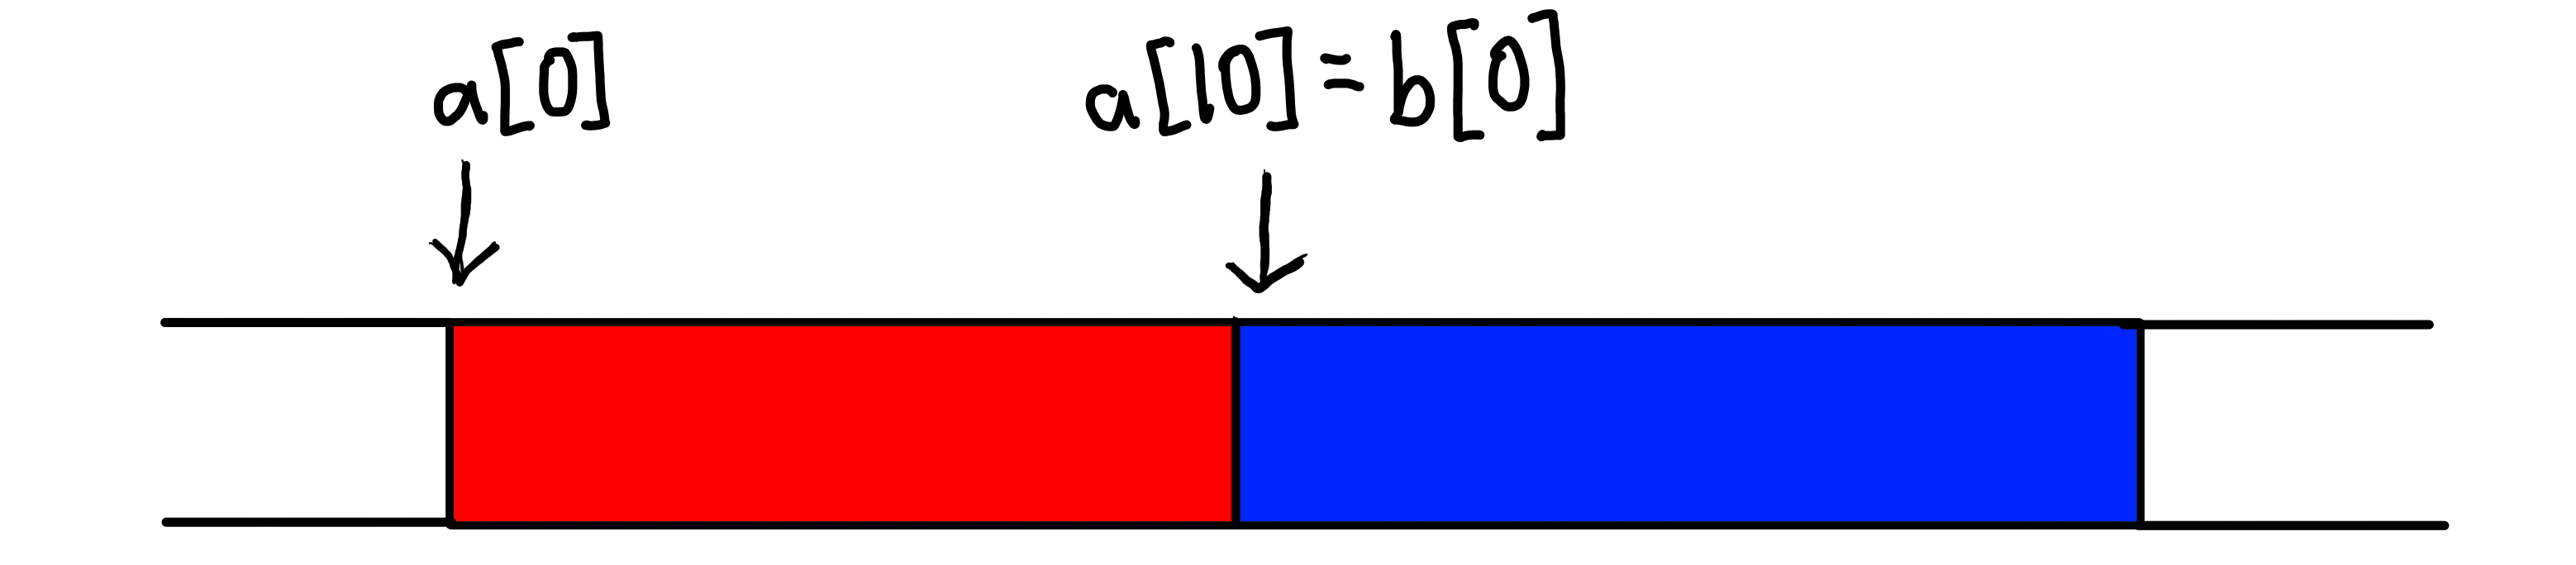
\includegraphics[width=.5\textwidth]{example.png}

To prevent the expression {\tt a[10] = 42} from overwriting {\tt b[0]}, we give {\tt a} and {\tt b}
unique {\it color tags} when they are allocated. In this case, we'll tag {\tt a} with \(\mathit{dyn ~ 0}\),
indicating that it's the first dynamically allocated object, and {\tt b} with \(\mathit{dyn ~ 1}\).
Then, when we evaluate the left-hand expression {\tt a} into its memory location \(l\), we tag
\(l\) with \(\mathit{dyn ~ 0}\). When we take the offset \(l + 10\), we keep that tag. And when we
perform the assignment, we check that the location tag at \(l\) matches. It doesn't, so we failstop.

The same principle applies for this code:

\vspace{\abovedisplayskip}
\begin{verbatim}
void main() {
  int* a = malloc(10 * sizeof(int));
  int* b = malloc(10 * sizeof(int));
  *(a + (b - a)) = 42;
}
\end{verbatim}
\vspace{\belowdisplayskip}

In this case, {\tt a} and {\tt b} could be allocated anywhere in the heap, and in Tagged C
the expression {\tt *(a + (b - a)) = 42} will always write to {\tt *b}. While this might be intentional
on the part of the programmer, it is also undefined behavior in the C standard, and in some
(but not all; see below) formal C semantics. Likewise, if {\tt a} and {\tt b} are next to each other
or in some other predictable arrangement, arithmetic like our first example can apply.
The memory safety policy works just the same in this scenario, with the tags being attached
by the call to malloc, once again using the \(\mathit{dyn}\) label in a global count of allocated blocks.
Meanwhile, values that are not derived from valid pointers at all are tagged \(X\), and can never
be read or written through, to avoid pointer forging, like this:

\vspace{\abovedisplayskip}
\begin{verbatim}
void main() {
  int* a = malloc(10 * sizeof(int));
  // We happen to know that a will be at address 1000
  *1000 = 42;
}
\end{verbatim}
\vspace{\belowdisplayskip}

Both stack and heap allocations use the \(\mathit{dyn}\) label and have a color that can grow arbitrarily
high. This is because over a program's execution, it might allocate an unbounded number of heap- or
stack-allocated objects, and each needs a unique identifier. Existing work has shown that in practice,
tag colors can be ``garbage collected'' and reused, but in Tagged C we assume them to be infinite and unique.

Lastly, we have global variables. While ``global safety'' is not as prominent a topic as heap or
stack safety, overrunning a global buffer is still a problem. It is also easy to forge a pointer to a global,
and when this happens it can undermine assumptions about the behavior of linked libraries whose globals
are not exported. Globals do not need dynamic colors, but can use their identifiers as tags, of the form
\(\mathit{glob} ~ id\).

\paragraph{Memory Safety: PVI and PNVI}

Our policies aim to enforce two memory models in particular: {\it PVI} (provenanace via integer) and
{\it PNVI} (provenance not via integer) from Memarian et al. \cite{???}. They propose PVI and PNVI
as memory models that support common idioms that are undefined in the C standard, but are still restrictive
enough as to support useful alias analysis for optimization. This application is orthogonal to
security, and violations of either memory model are treated as undefined behavior, just as in the
C standard. Our goal is to turn that UB into failstop behavior, so that undefined programs cannot accidentally
undermine their own security.

Both memory models represent pointers as integers, just as Tagged C does, with additional provenance
associated with each object. An integer cast to a pointer in PVI retains this provenance, enabling
integer operations to be performed on it prior to it being cast back to a pointer.
In PNVI, by contrast, an integer cast to a pointer gains the provenance of the object it points
to when the cast occurs. While PNVI supports a wider range of programs, it is inconsistent with important
assumptions of the C memory model, in ways that may have serious security consequences.
The difference between PVI and PNVI is illustrated in Figure \ref{fig:PVI-PNVI}.

\begin{figure}
  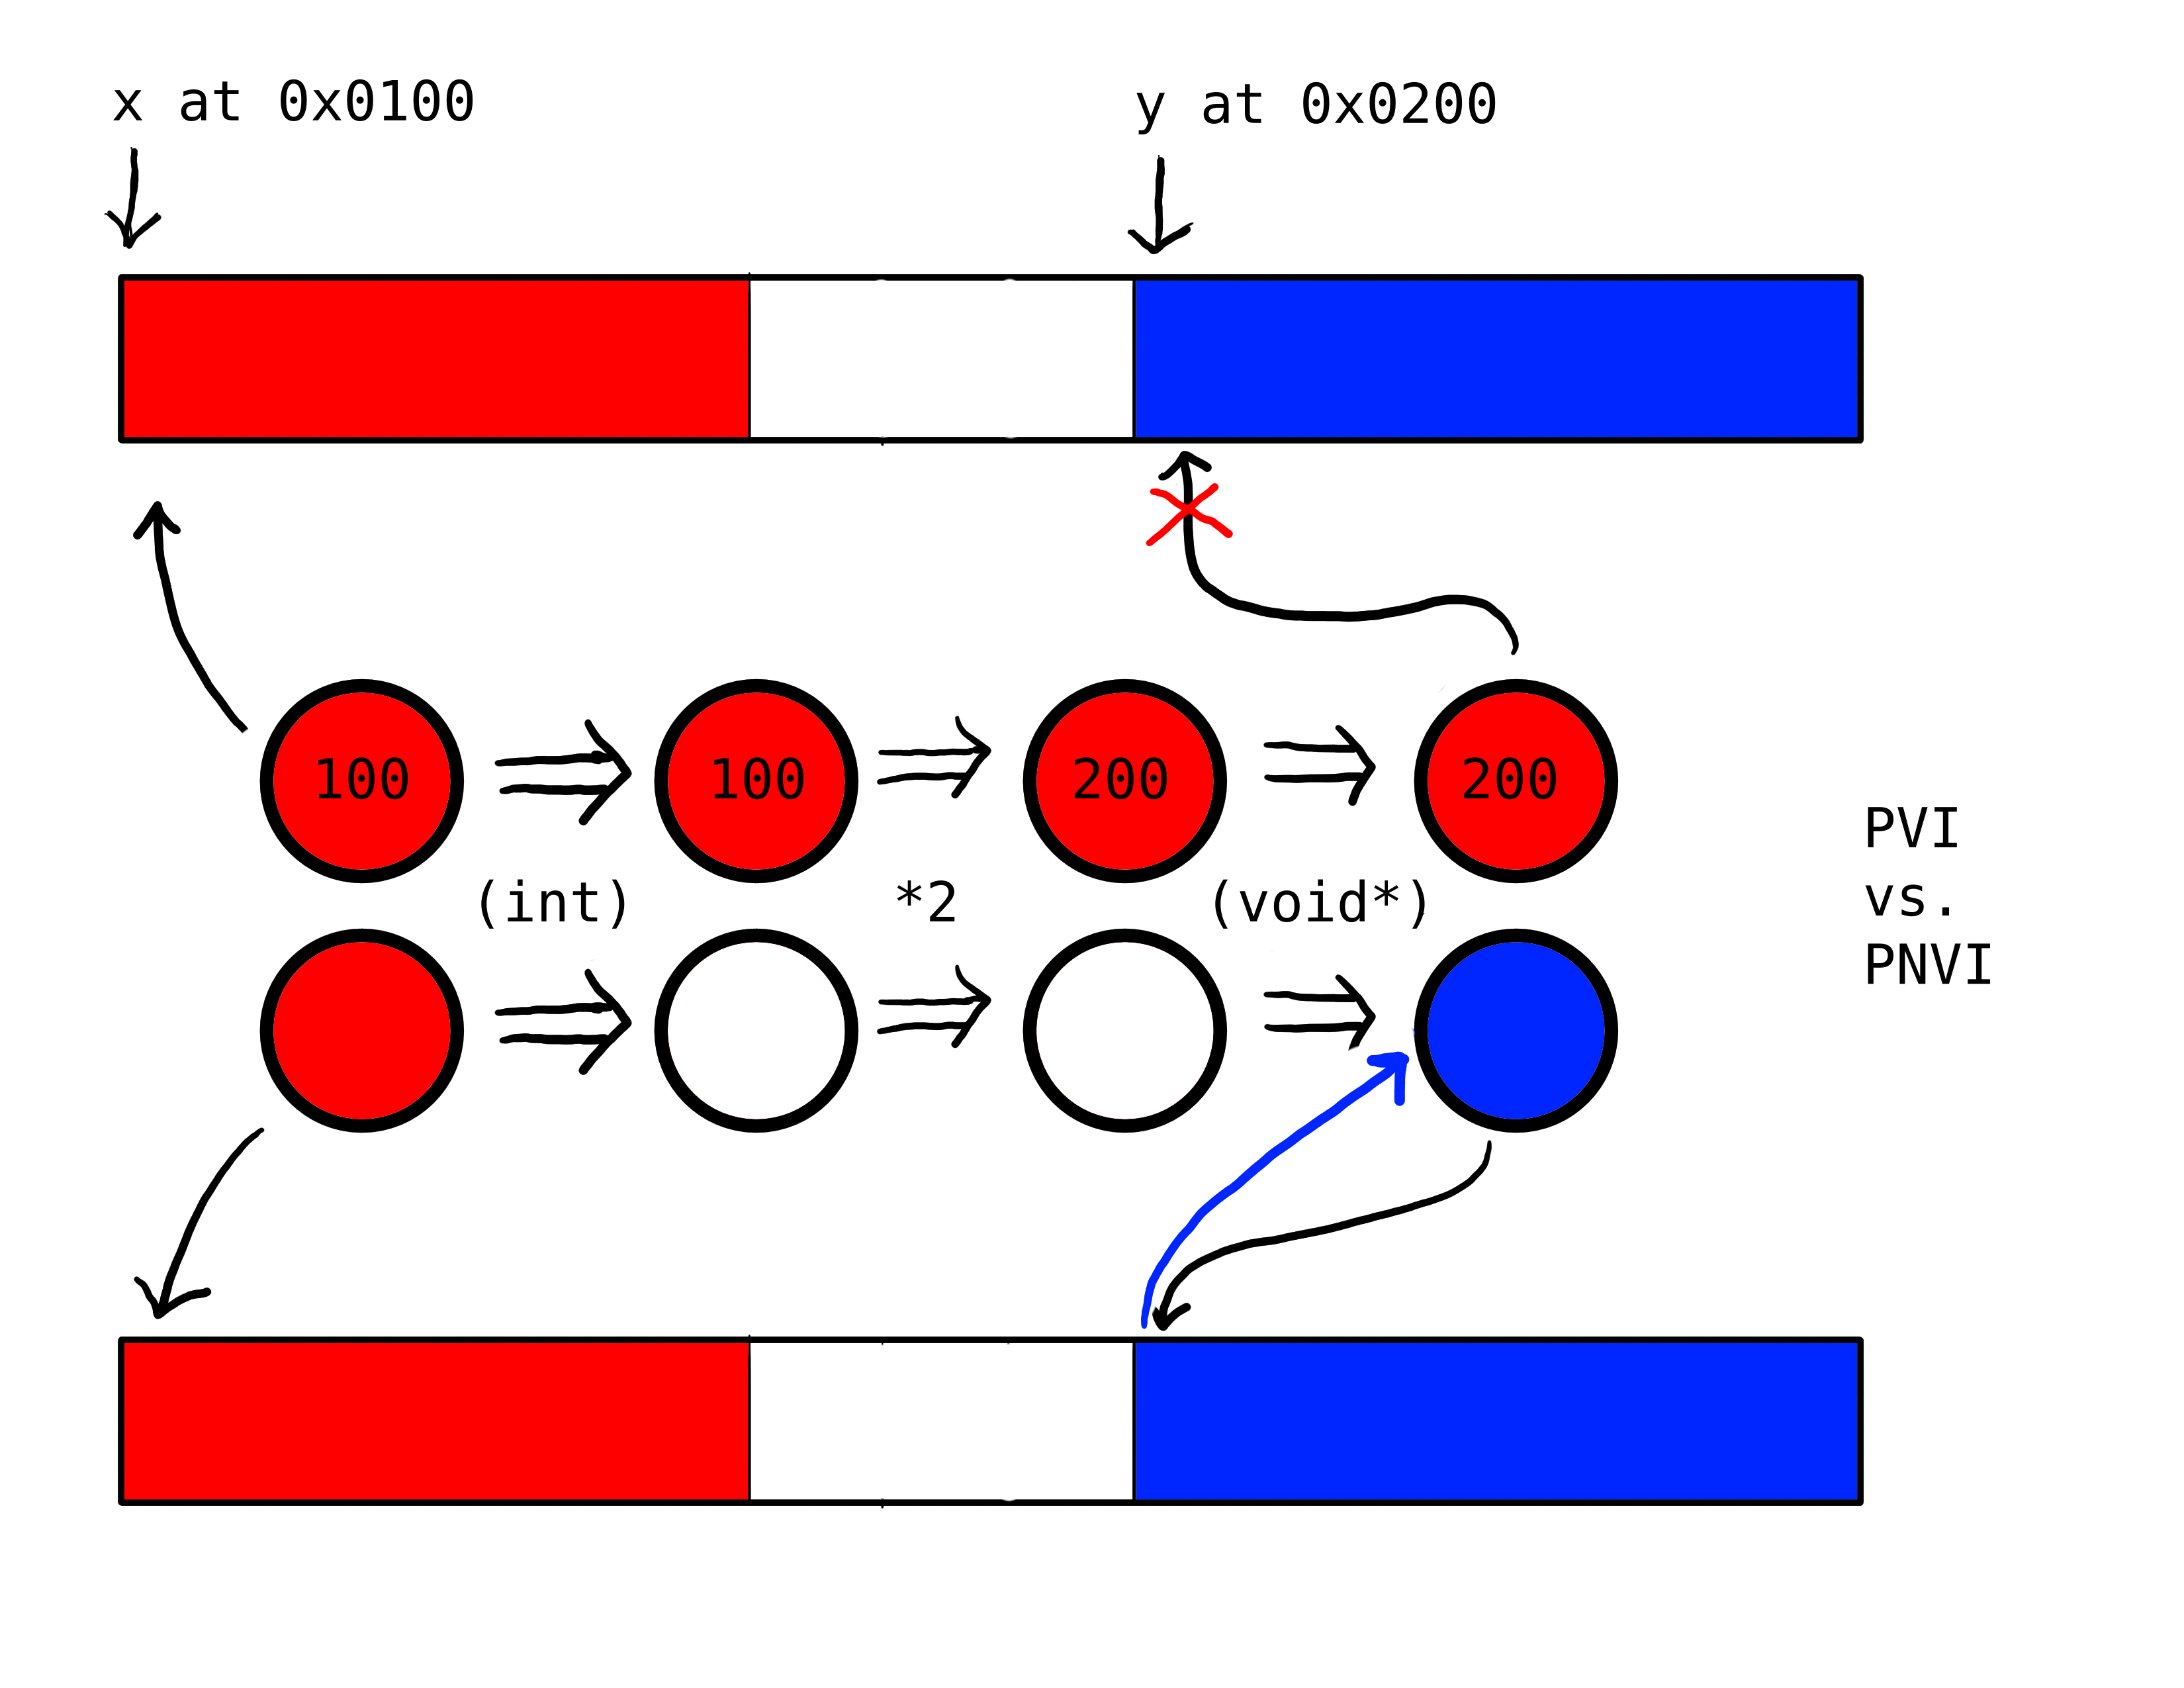
\includegraphics[width=.6\textwidth]{PVIvsPNVI.png}
  \caption{Integer-pointer casts in PVI and PNVI}
  \label{fig:PVI-PNVI}
\end{figure}

We will aim to prove that for any program, if it is run in both the PVI semantics
and in Tagged C with our PVI policy, it either produces identical output, or it is both
undefined in the PVI semantics and failstops in Tagged C. Likewise for PNVI, except that
some UB in PNVI is non-deterministic, and we only require that it failstop in an execution
that would {\it reach} the UB.

\subsection{PVI Definitions}

Here we give the relevant tag rules for the PVI policy, and describe the control points that
they attach to. We will, for each rule, first give the control point(s) that use it, along
with a brief explanation of what the surrounding semantics rules do, and then give the rule.
For these policies, all control points appear in expression reduction steps.
The machine state consists of the PC tag \(\PCT\), a memory \(\mem\),
the global environment \(\genv\), and a local environment \(\lenv\). These are contextual semantics,
so each expression is situated in some context \(\mathit{ctx}\).

The core of the PVI policy is the {\it provenance color}, represented
by a natural number.
%
\begin{align*}
  T ::= & \mathit{glob} ~ id & id \in \mathit{ident} \\
  & \mathit{dyn} ~ \tagcolor & \tagcolor \in \mathbb{N} \\
\end{align*}

\paragraph*{Color generation}

New colors are generated when objects are allocated. When exactly that occurs
depends on where the object lives. Global variables are a special case: they are
allocated during program initialization, before execution begins. As such they
do not have a control point per se, but a rule that functions similarly, while
being more expressive.

%All of our allocation control points differ from the normal ones in that they
%pass a type as a parameter and recieve a list of tags that they apply to
%a memory region of the size of that type.

Given a list \(xs\) of variable identifiers \(id\) and types
\(ty\), a program's initial memory is defined by iteratively allocating each one
in memory and updating the global environment with its base address, bound, type,
and a static identity tag. Let \(|ty|\) be a function from types to their sizes
in bytes. The memory is initialized \(\vundef@\vt@\overline{\lt}\)
for some \(\vt\) and \(\overline{\lt}\), unless given an initializer.
Let \(\mem_0\) and \(\genv_0\) be the initial (empty) memory and environment.
The parameter \(b\) marks the start of the global region.

%Since we don't need to initialize tags in memory dynamically, our rule for
%selecting these tags can cover the entire initialization of the memory with arbitrary
%granularity. We represent this as a list of tags of length \(|ty|\).

\[\mathit{globals} ~ xs ~ b =
\begin{cases}
  (\mem_0, \genv_0) & \textnormal{if } xs = \varepsilon \\
  (\mem[p \dots p+|ty| \mapsto \vundef@\vt@\overline{\lt}]_{|ty|}, & \textnormal{if } xs = (id,ty)::xs' \\
  ~ \genv[id \mapsto (\mathit{p, p+|ty|,ty,\pt})]) & \textnormal{and } \trule{\globaltres}{\globalt} \\
  & \textnormal{where } (\mem,\genv) = \mathit{globals} ~ xs' ~ (b + |ty|) \\
\end{cases}\]

\[\begin{aligned}
\truledef{\globalt}
\settag{\pt}{\mathit{glob ~ id}}
\settag{\vt}{X}
\settag{\overline{\lt}}{\left[\mathit{glob} ~ id \mid 0 \leq i < s\right]}
\end{aligned}\]

Stack-allocated locals are allocated at the start of a function call. Like a global environment,
a local environment maps indentifiers to base, bound, type, and tag. The rule is almost identical
to allocation of globals, except that the stack allocator, \(\mathit{stack\_alloc}\) will be more
complex in order to support deallocation (in practice, it uses a normal stack structure and allocates
and deallocates by increasing and decreasing a ``stack pointer''.)

Since allocations occur at runtime, the value and location tags that initialize the allocated memory
are optional. They would be realized by initializing the entire allocated object at allocation-time,
which adds linear overhead if the object was not otherwise being initialized.

\[\mathit{locals} ~ xs ~ \mem ~ \lenv =
\begin{cases}
  (\mem, \lenv) & \textnormal{if } xs = \varepsilon \\
  \mathit{locals} ~ xs' ~ \mem'' ~ \lenv' & \textnormal{if } xs = (id,ty)::xs' \\
  & \textnormal{where } (\mem',p) \leftarrow \mathit{stack\_alloc} ~ |ty| ~ \mem, \\
  & \mem'' = \mem'[p \dots p+|ty| \mapsto \vundef@\vt@\overline{\lt}]_{|ty|}, \\
  & \trule{\localtres}{\localt}, \\
  & \textnormal{and } \lenv' = \lenv[id \mapsto (\mathit{p, p+|ty|,ty,\pt})]) \\
\end{cases}\]
              
In the tag rule, the PC Tag carries the ``next'' color to be assigned. We mark both the pointer tag
(which is stored in the local environment) with that color, along with the location tags on the
allocated memory. Then we increment the PC Tag to give the next allocation a unique color.

\[\begin{aligned}
\truledef{\localt}
\settag{\pt}{dyn ~ \PCT}
\settagopt{\vt}{X}
\settagopt{\overline{\lt}}{\left[dyn ~ \PCT \mid 0 \leq i < s\right]}
\settag{\PCT'}{\PCT+1}
\end{aligned}\]
         
Heap objects are the most interesting: they are allocated via calls to malloc.
In Tagged C, malloc is modeled as an external call to a built-in, so this takes the form
of a special case of that expression. Where \(\mathit{heap\_alloc}\) is some allocation
function (a parameter of the memory model) that takes a size and a memory and returns an address:

\allocstep

And the tag rule is identical to \(\mathbf{LocalT}\), except that it always treats the allocated
object as an array of bytes (making the location tags are always identical.)

\[\begin{aligned}
\truledef{\malloct}
\settag{\pt}{dyn ~ \PCT}
\settagopt{\vt}{X}
\settagopt{\overline{\lt}}{\left[dyn ~ \PCT\right]}
\settag{\PCT'}{\PCT + 1}
\end{aligned}\]

\paragraph*{Color Checking}

When we perform a memory load or store, we check that the pointer tag on the left hand
of the assignment matches the location tag on all of the bytes being loaded or stored.
For instance, in a normal {\it valof} expression, which accesses a left-hand value:

\valofstep

We want to both check that the pointer tag matches all of the location tags, and propagate the
value tag on the value in memory alongside that value.

\[\begin{aligned}
\truledef{\loadt}
\assert{\forall \lt \in \overline{\lt} . \pt = \lt}
\settag{\vt'}{\vt}
\end{aligned}\]

There are two other expressions that load from memory, and which therefore invoke
this same rule, {\it assignop} and {\it postincr}. Note that the C spec has the order
of evaluation for {\it assignop} ``unsequenced''; I follow CompCert in evaluating both the left
and right completely before performing the load. Intuitively, assignment-with-an-operator is
classed along with the standard assignment in the spec, so it is appropriate that it be ordered
in the same way.

\assignopstep

\postincstep

On the flip side, we store values to memory using the {\it assign} expression:

\assignstep

As before, we check that the pointer tag matches the locations tags, and then propagate the
value tag (ignoring and overwriting the original value tag.) In addition, we propagate the PC Tag.
                  
\[\begin{aligned}
\truledef{\storet}
\assert{\forall \lt \in \overline{\lt} . \pt = \lt}
\settag{\PCT'}{\PCT}
\settag{\vt'}{\vt_2}
\settag{\overline{\lt'}}{\overline{\lt}}
\end{aligned}\]

\paragraph*{Color Propagation}

When a value moves from one location to another, it carries the same tag.
We already saw this in the load and store rules: they maintain the relationship
between the pointer and its tag. Of note here is the \(\mathbf{VarT}\) control point,
which transmits the pointer tag from the environment onto the location expression.
In this policy, it propagates the color unchanged.

\varstep

%In PVI semantics, a pointer cast to an integer maintains its provenance, so the
%cast rule should not change its tag. When cast in this way, integer operations
%are defined on them. Our semantics convert a pointer value to an integer and back
%on cast.

Then the color is propagated via all unary operations and all binary operations
where exactly one argument has a color. Performing an operation with two values
with color tags (i.e., two cast pointers) clears the tag on the result. It can still
be used as an integer, but if cast back to a pointer it will be invalid.

\unopstep

\binopstep

\vspace{\abovedisplayskip}
            
\begin{minipage}[t]{.49\textwidth}            
  \[\begin{aligned}
  \truledef{\unopt}
  \settag{\PCT'}{\PCT}
  \settag{\vt'}{\vt}
  \end{aligned}\]
\end{minipage}
\begin{minipage}[t]{.49\textwidth}           
  \[\begin{aligned}
  \truledef{\binopt}
  \settag{\PCT'}{\PCT}
  \settag{\vt'}{\caseof{(\vt_1,~ \vt_2)}}
  \caseentry{\mathit{dyn ~ n},X}{\mathit{dyn ~ n}} \\
  \caseentry{\mathit{glob ~ id},X}{\mathit{glob ~ id}} \\
  \caseentry{X,t}{t} \\
  \end{aligned}\]
\end{minipage}

\subsection{PNVI Definitions}

In PNVI, the basic provenance model remains the same as PVI, so we can reuse most of the
same rules. The primary difference is what happens when we cast a pointer to an integer.
In PVI, tags are propagated as normal.

To support PNVI, we need the {\it cast} expression to update the tags of a pointer
being cast to an integer and vice versa. We add two special-case steps to reflect this.

\judgmenttwo{\optional{\(\mem[p]_{|ty|} = \_@\vt_2 @ \overline{\lt}\)}}
            {\(\trule{\picasttres}{\picastt}\)}
            {\(\defestate{\cast{int}{\val{p}{\pt}}}{\tptr{ty}} \longrightarrow
              \defestate{\val{p}{vt}}{int}\)}

\judgmenttwo{\optional{\(\mem[p]_{|ty|} = \_@\vt_2 @ \overline{\lt}\)}}
            {\(\trule{\ipcasttres}{\ipcastt}\)}
            {\(\defestate{\cast{int}{\val{p}{\pt}}}{\tptr{ty}} \longrightarrow
              \defestate{\val{p}{vt}}{int}\)}

For casting an integer to a pointer, we don't need the optional ``peek'' at the memory that it points to.
We simply clear the tag on the resulting integer.
\[\begin{aligned}
\truledef{\picastt}
\settag{\PCT'}{\PCT}
\settag{\vt}{X}
\end{aligned}\]

On the other hand, when casting back to a pointer, we need to check the color
of the object that it points to.

\[\begin{aligned}
\truledef{\ipcastt}
\assert{\exists t . \forall \lt \in \overline{\lt} . \lt = t \land t \not = X}
\settag{\PCT'}{\PCT}
\settag{\pt}{t}
\end{aligned}\]

\paragraph{Realizing the Integer-Pointer Cast}

The pointer cast rules take as input the tags on the location pointed to by the
argument being cast. This requires the compiler to add extra instructions to retrieve that tag.
On RISCV, the sequence would be as follows, assuming that {\tt a0} contains the
value being cast. The meaning of instruction tags will be explained below.

\begin{verbatim}
lw a1 a0 0 @ RETRIEVE
sub a1 a1 a1 @ L
add a0 a1 a0 @ IPCAST
\end{verbatim}

In the underlying assembly, we use instruction tags to inform the low-level monitor
of the purpose of each instruction. {\tt RETRIEVE} indicates a special load
whose job is retrieve value and location tags from a location in memory. When it sees
a {\tt RETRIEVE} tag, the monitor allows the load even if it should failstop under the
Concrete C backstop policy. If the load should failstop, however, it is given a default
tag rather than the tags on the memory. A legal load recieves both the value and the location
tags.

The {\tt L} instruction tag simply denotes taking the left-operand's tag on the result of a
binary operation. In this case both operations are identical, but we still need to pick one.
Finally, the {\tt IPCAST} tag declares that this instruction should mimic the Tagged-C-level
rule.

\section{Secure Information Flow}
\label{sec:SIF}

To motivate our next policy, let's consider an erroneous piece of code:

\begin{verbatim}
void sanitize(src, dst);
char* sql_query(char* query);

void get_data(char* name, char* buf, int field) {
  // field: 1=address, 2=phone, default=astrological sign
  char[10] name_san;
  char[100] query;
  sanitize(name, name_san);

  switch(field) {
    case 1:
      sprintf(query, "select address where name =");
      strncat(query, name_san, strlen(name_san));
      break;
    case 2:
      sprintf(query, "select phone where name =");
      strncat(query, name_san, strlen(name_san));
      break;
    default:
      sprintf(query, "select sign where name =");
      strncat(query, name, strlen(name)); // Oops!
      break;
  }

  sprintf(buf, sql_query(query);
  return;
}
\end{verbatim}

This function sanitizes its input {\tt name}, then appends the result to an appropriate SQL
query, storing the result in {\tt buf}. But, in the default case, the programmer has accidentally
used the unsanitized string! This creates the opportunity for an SQL injection attack: a caller
to this function could (presumably at the behest of an outside user) call it with {\tt field} of
3 and {\tt name} of ``Bobby; drop table;''.

We model this as a form of {\em secure information flow} (SIF), a variant of
{\em information flow control} (IFC), as described in the venerable Denning and Denning
\cite{denning1977:SecureInformationFlow}.
Specifically, this is an {\it intransitive} SIF setting: we wish to allow {\tt name} to influence
the result of {\tt sanitize}, naturally, and the result of {\tt sanitize} to influence the
value passed to {\tt sql\_query}, but we do not wish for {\tt name} to influence {\tt sql\_query}
directly.

SIF is specified by a set of flow rules between what we will term {\em sources} and {\em sinks}.
A source \(\sigma\) can be an argument of a function, its return value, or a global.
A sink \(\psi\) can additionally be the set of heap objects allocated by a given function.
We write these as follows:

\begin{minipage}{0.5\textwidth}
  \[\begin{aligned}
  \sigma ::= & x & \textnormal{Global} \\
  & f(x) & \textnormal{Argument {\tt x} of {\tt f}} \\
  & f.ret & \textnormal{Return value of {\tt f}} \\
  \end{aligned}\]
\end{minipage}
\begin{minipage}{0.5\textwidth}
  \[\begin{aligned}
  \psi ::= & x & \textnormal{Global} \\
  & f(x) & \textnormal{Argument {\tt x} of {\tt f}} \\
  & f.ret & \textnormal{Return value of {\tt f}} \\
  & f.m & \textnormal{Memory owned by {\tt f}} \\
  \end{aligned}\]
\end{minipage}

In classic SIF theory, we specify an {\em information flow policy} (IFPol)---not to be confused with a
tag policy---as a relation \(\cdot \rightsquigarrow \cdot \in \sigma \times \psi\). However,
manually defining such a policy is challenging, especially in an intransitive setting.
We envision the IFPol being initially stated in negative terms, with the ``no-flow'' relation
\(\not \rightsquigarrow\). That is, we will assume by default that for any source \(\sigma\)
and any sink \(\psi\), \(\sigma \rightsquigarrow \psi\), unless the user has explicitly
declared the contrary.

So, in the above example, the user would declare that \(\mathtt{name} \not \rightsquigarrow \mathtt{sql\_query}\).
But, in the case of \(\mathtt{sanitize}\), we want it to be the case that \(\mathtt{name}\) can flow to
\(\mathtt{sql\_query}\) only via \(\mathtt{sanitize}\). We therefore need to allow the user to declare
a {\em declassification} rule. In general we will write \(\sigma / \sigma'\) to indicate that \(\sigma'\)
supersedes \(\sigma\): if a value that has been influenced by \(\sigma\) influences \(\sigma'\), we
can safely ignore its history with \(\sigma\). We may write \(* / \sigma\) to say that \(\sigma\)
declassifies anything.

For example, suppose that in the following code, we want to enforce a no-flow rule between
the argument {\tt x} of {\tt f} and the global variable {\tt z}
(\(\mathtt{f.x} \not \rightsquigarrow \mathtt{z}\)), and a declassification rule
\(* / \mathtt{g.a}\).

\begin{verbatim}
  int z;

  int g(int a);

  void f(int x, int y) {
    z = x;                    // violation
    z = x + y;                // violation
    if(x) z = 1; else z = 0;  // violation
    z = g(x);                 // violation, unless f.x / g.a
  }
\end{verbatim}

The first three lines of {\tt f} violate the no-flow relation by storing values derived from
{\tt x} into {\tt z}. The third line is especially interesting: although {\tt x} is not stored
directly, the value that is stored is conditioned upon it, and can be used to deduce information
about the original value. This is termed an {\em implicit flow}. Finally, in the last line,
the value of {\tt g(x)} depends on {\tt x}, which is a violation unless it is subject to a
declassification rule.

We can therefore define an IFPol as a set of rules of each kind:

\[I \subseteq \{\sigma \not \rightsquigarrow \psi \mid \sigma \not \eq \psi\} \cup
\{\sigma / \sigma' \mid \sigma \not \eq \sigma'\}\]

We do not need to distinguish between rules that notionally represent ``integrity'' versus ``confidentiality''
concerns. The SQL injection example is an instance of integrity, ensuring that an input cannot influence data
in an undesired way, but the same concept can be used to prevent data from influencing the program's output
inappropriately.

\paragraph{SIF, formally}

We can characterize the protection offered by a SIF policy in terms of a {\em non-interference}
property along the lines of Bay and Askarov \cite{}. We annotate our transitions with events \(\alpha\),
each representing the transmission of a value through a source or sink---possibly several. We write the
projection of data relevant to a particular source \(\sigma\) or sink \(\psi\) as \(\pi_\sigma(\alpha)\)
or \(\pi_\psi(\alpha)\).

\[\begin{aligned}
\alpha ::= & \\
& \\
\end{aligned}\]

[TODO: add the relevant events to their transitions in the semantics.]

Now, we define the knowledge that an observer monitoring a particular sink can extrapolate about the
state of the system as a whole, as a set of states that are consistent with the events it observes.
Given some initial state \(S\), this is precisely the set of other initial states that might
produce the same trace (or an extension thereof) and that are equivalent.

\[\mathbf{K}(S,\overline{\alpha},\sigma,\psi) \triangleq
\{S' \mid S \sim_\sigma S' \land S' \hookrightarrow_{\psi} \overline{\alpha} \cdot \alpha\}\]

Then, absent any declassification rules, we can define non-interference as holding between
\(\sigma\) and \(\psi\) if, for any states \(S_1\) and \(S_2\) such that
\(S_1 \xrightarrow{\overline{\alpha}\cdot \alpha} S_2\),
\(\mathbf{K}(S_2,\overline{\alpha}\cdot \alpha,\sigma,\psi) \supseteq
\mathbf{K}(S_1,\overline{\alpha},\sigma,\psi)\). That is, every world that was possible before
\(\alpha\) remains possible after.

In the presence of declassification, we add an exception for the case where \(\alpha\)
reflects an event that should indeed allow an observer to gain some information. We extend
the above definition to talk about all of \(I\).

\[NI_I \triangleq \forall S_1, S_2, \overline{\alpha}, \alpha .
\begin{cases}
\mathbf{K}(S_2,\overline{\alpha}\cdot \alpha,\sigma,\psi) \supseteq
\mathbf{K}(S_1,\overline{\alpha},\sigma,\psi) &
\textnormal{if } \sigma \not \rightsquigarrow \psi \in I \\
\mathbf{K}(S_2,\overline{\alpha}\cdot \alpha,\sigma,\psi) \supseteq
\mathbf{K}(S_1,\overline{\alpha},\sigma \sqcup \sigma',\psi &
\textnormal{if } \sigma / \sigma' \in I \land \sigma' \rightsquigarrow \psi \in I \\
\end{cases}\]

\paragraph{Tagging SIF}

We track the influence of a particular source, or its ``taint,'' through the system in the form
of tags on values. A value that is tagged \(\mathit{vtaint} ~ \overline{\sigma}\) has been influnced
by all of the sources in \(\overline{\sigma}\). We also define a set of tags that indicate that a
particular function argument or the memory location of an object represents a sink that is the
target of one or more no-flow rules. If a sink \(\psi\) is tagged
\(\mathit{forbid} ~ \overline{\sigma}\), then for all \(\sigma \in \overline{\sigma}\),
\(\sigma \not \rightsquigarrow \psi\) must be in our IFPol. Finally, the PC Tag must carry additional
information: when the PC Tag is tainted, it must keep a record of the scope of the taint, in the form
of a label. We will explain below how this scope is computed.
%
\begin{align*}
  T ::= & \mathit{vtaint} ~ \overline{\sigma} \\
  & \mathit{forbid} ~ \overline{\sigma} \\
  & \mathit{pctaint} ~ \overline{(L,\sigma)} \\
\end{align*}
%
We define four important operations on tags: {\em join} (\(t_1 \sqcup t_2\)), {\em bounded join}
(\(t_1 [L \rightarrowtail t_2]\)), {\em minus} (\(t_1 - t_2\)), and {\em check} (\(t_1 \models t_2\)),
all partial functions.
%
\[t_1 \sqcup t_2 \triangleq
\begin{cases}
  \mathit{vtaint} ~ (\overline{\sigma}_1 \cup \overline{\sigma}_2) &
  \textnormal{if } t_1 = \mathit{vtaint} ~ \overline{\sigma}_1 \textnormal{ and }
  t_2 = \mathit{vtaint} ~ \overline{\sigma}_2\\
  \mathit{vtaint} ~ (\overline{\sigma}_2 \cup \{\sigma \mid (L,\sigma) \in \overline{(L,\sigma)}_1\}) &
  \textnormal{if } t_1 = \mathit{pctaint} ~ \overline{(L,\sigma)}_1 \textnormal{ and }
  t_2 = \mathit{vtaint} ~ \overline{\sigma}_2\\
  \mathit{vtaint} ~ (\overline{\sigma}_1 \cup \{\sigma \mid (L,\sigma) \in \overline{(L,\sigma)}_2\}) &
  \textnormal{if } t_2 = \mathit{pctaint} ~ \overline{(L,\sigma)}_2 \textnormal{ and }
  t_1 = \mathit{vtaint} ~ \overline{\sigma}_1\\
  \bot & \textnormal{otherwise} \\
\end{cases}\]
%
\[L \rightarrowtail t_1 \sqcup t_2 \triangleq
\begin{cases}
  \mathit{pctaint} ~ (\overline{\sigma}_1 \cup \overline{\sigma}_2) &
  \textnormal{if } t_1 = \mathit{vtaint} ~ \overline{\sigma}_1 \textnormal{ and }
  t_2 = \mathit{vtaint} ~ \overline{\sigma}_2\\
  \bot & \textnormal{otherwise} \\
\end{cases}\]
%
\[t - \sigma \triangleq
\begin{cases}
  \mathit{taint} ~ (\overline{\sigma}' - \sigma) &
  \textnormal{if } t = \mathit{taint} ~ \overline{\sigma}' \\
  \bot & \textnormal{otherwise} \\
\end{cases}\]
%
\[t_2 \models t_1 \triangleq
\begin{cases}
  \mathbf{t} & \textnormal{if } t_1 = \mathit{taint} ~ \overline{\sigma}_1,
  t_2 = \mathit{forbid} ~ \overline{\sigma}_2, \textnormal{ and }
  \overline{\sigma}_1 \cap \overline{\sigma}_2 = \emptyset \\
  \mathbf{f} & \textnormal{if } t_1 = \mathit{taint} ~ \overline{\sigma}_1,
  t_2 = \mathit{forbid} ~ \overline{\sigma}_2, \textnormal{ and }
  \overline{\sigma}_1 \cap \overline{\sigma}_2 \not = \emptyset \\
  \bot & \textnormal{otherwise} \\
\end{cases}\]

\paragraph{Tainting and Checking Arguments and Returns}

Now we can begin to give our policy, given an arbitrary IFPol \(I\).

A function argument or return value can be either a source or a sink.
So, when they are processed by the {\em call-state} and {\em return-state} rules,
we must both check that the value being passed or returned is not tainted by a forbidden
source, and then add the current source to its taint.
The call-state rule executes at the beginning of a call, moving all of its arguments into
the local environment, using the \(\mathbf{ArgT}\) tag rule.
The return-state rule executes after the call returns, inserting the result into the
context saved in the continuation. The program counter on return and the result's tag are
set by the \(\mathbf{CallerRetT}\) tag rule. Both are given in \cref{fig:callretsteps}.

\begin{figure}
  \callstep
  \returnstep
  \caption{Call and Return Steps}
  \label{fig:callretsteps}
\end{figure}
  
\begin{minipage}[t]{.49\textwidth}            
  \[\begin{aligned}
  \truledef{\argt}
  \letin{t := \mathit{forbid} ~ \{\sigma \mid \sigma \not \rightsquigarrow f(x) \in I\}}
  \assert{t \models \PCT \sqcup \vt}
  \letin{\vt_1 := \vt - \{\sigma \mid \sigma / f(x) \in I \}}
  \letin{\vt_2 := \vt_1 \sqcup \mathit{tainted} ~ \{f(x)\}}
  \settag{\vt'}{\vt_2}
  \end{aligned}\]
\end{minipage}
\begin{minipage}[t]{.49\textwidth}            
  \[\begin{aligned}
  \truledef{\callerrett}
  \letin{t := \mathit{forbid} ~ \{\sigma \mid \sigma \not \rightsquigarrow f.ret \in I\}}
  \assert{t \models \PCT \sqcup \vt}
  \letin{\vt_1 := \vt - \{\sigma \mid \sigma / f.ret \in I \}}
  \letin{\vt_2 := \vt_1 \sqcup \mathit{tainted} ~ \{f.ret\}}
  \settag{\vt'}{\vt_2}
  \end{aligned}\]
\end{minipage}

Global variables are also possible sources or sinks. In this case, we initialize their
tags to carry this information.
\[\begin{aligned}
\truledef{\globalt}
\settag{\pt}{\mathit{tainted} ~ \emptyset}
\settag{\vt}{\mathit{tainted} ~ \{x\}}
\settag{\overline{\lt}}{\left[\mathit{forbidden} ~ \{\sigma \mid x \not \rightsquigarrow x \in I\}\right]}
\end{aligned}\]

\paragraph{Introducing Dynamic Sinks}

One scenario that does not really match the others is when the sink is dynamically allocated
memory. In this case, we need to tag the memory at allocation-time with the forbidden
sources.

\[\begin{aligned}
\truledef{\malloct}
\settag{\pt}{\PCT \sqcup \mathit{tainted} ~ \emptyset}
\settagopt{\vt}{\mathit{tainted} ~ \emptyset}
\settagopt{\overline{\lt}}{\left[\mathit{forbidden} ~ \{\sigma \mid \sigma \not \rightsquigarrow f.m\} \right]}
\settag{\PCT'}{\PCT + 1}
\end{aligned}\]

\paragraph{Propagating Taint Through Expressions}

It is simple enough to determine when a value is tainted: at a function
call, all function arguments are tagged with their source identity, and the result
of any expression is tagged with the union of the sources of its operands. If the
expression involves a store or function call itself, we must check the taints on
the value being stored or passed against the forbidden list of the target.

Unary and binary operations:

\begin{minipage}[t]{.49\textwidth}
  \[\begin{aligned}
  \truledef{\unopt}
  \settag{\vt'}{\vt}
  \end{aligned}\]
\end{minipage}
\begin{minipage}[t]{.49\textwidth}
  \[\begin{aligned}
  \truledef{\binopt}
  \settag{\vt'}{
    \vt_1 \sqcup \vt_2
  }
  \end{aligned}\]
\end{minipage}

Loads and stores:

\begin{minipage}[t]{.4\textwidth}
\[\begin{aligned}
\truledef{\loadt}
\settag{\vt'}{\PCT \sqcup \pt \sqcup \vt}
\end{aligned}\]
\end{minipage}
\begin{minipage}[t]{.59\textwidth}
\[\begin{aligned}
\truledef{\storet}
\assert{\forall \lt \in \overline{\lt} . \lt \models \PCT \sqcup \pt \sqcup \vt_2}
\settag{\PCT'}{\PCT}
\settag{\vt'}{\PCT \sqcup \pt \sqcup \vt_2}
\settag{\overline{\lt'}}{\overline{\lt}}
\end{aligned}\]
\end{minipage}

\paragraph{Implicit Flows}

Things become trickier when the program's control-flow itself can be tainted. This can occur in
any of our semantics' steps that can produce different statements and continuations
depending on the tained value. At that point, any change to the machine state constitutes
an information flow.

To be more specific, consider a statement that contains an expression, \(\stmt(\expr)\),
such that when filled in with a tainted value:
%
\[\sstate{\PCT}{\mem}{\genv}{\lenv}{\stmt\val{v_1}{\mathit{taint} ~ \sigma}}{\cont} \longrightarrow
\sstate{\PCT_1}{\mem_1}{\genv_1}{\lenv_1}{\stmt_1}{\cont_1}\]
%
while
%
\[\sstate{\PCT}{\mem}{\genv}{\lenv}{\stmt\val{v_1}{\mathit{taint} ~ \sigma}}{\cont} \longrightarrow
\sstate{\PCT_2}{\mem_2}{\genv_2}{\lenv_2}{\stmt_2}{\cont_2}\]
%
and where \(\stmt_1 \not = \stmt_2\) or \(\cont_1 \not = \cont_2\). Taking either step
should taint the program state itself! We represent this as a taint on the PC Tag.
When the PC Tag is tainted, all stores to memory and all updates to environments must
also be tainted until all branches eventually rejoin.
We term the point at which it is safe to remove taint a {\it join point}.
In terms of the program's control-flow graph, the
join point of a branch is its immediate post-dominator.

In many simple programs, the join point of a conditional or loop is obvious:
the point at which the chosen branch is complete, or the loop has ended.
Such a simple example can be seen in \cref{fig:ifthenelse}; {\tt public1} must be
tagged with the taint tag of {\tt secret}, while it is safe to tag {\tt public2}
\(X\), because that is after the join point, {\tt J}. The same goes for \cref{fig:while},
because we are in a {\em termination-insensitive} setting \cite{}. This means that we
consider only terminating runs. So, we can guarantee that the post-dominator \(J\)
of the while loop is reached.

But in the presence of unrestricted go-to statements, a join point may not be
local---and sometimes may not exist within the function, assuming that we have not
consolidated return points. Consider \cref{fig:forbreak}, which
uses go-to statements to create an approximation of an if-statement whose join-point
is far removed from the for-loop. The label {\tt J} now has nothing to do with the
semantics of any particular statement.

Luckily this can still be determined statically from a function's full
control-flow graph. So, to implement the policy, we must first transform our program
by adding labels at the join point of each conditional.
Every statement that branches carries an optional label indicating its corresponding
join point. If it doesn't have such
a label, that indicates that there is no join point within the function---once the PC Tag is tainted,
it must remain so until a return.

\begin{figure}
  \begin{subfigure}{0.5\textwidth}
\begin{verbatim}
int f(bool secret) {
    int public1, public2;

S:  if (secret) {
b1:     public1 = 1;
    } else {
b2:     public1 = 0;
    }

J:  public2 = 42;

    return public2;
}
\end{verbatim}
  \end{subfigure}
  \begin{subfigure}{0.5\textwidth}
    \begin{tikzpicture}
      [ initial text={}, initial distance=4em,
        accepting/.style=accepting by arrow,
        accepting distance=4em
      ]
      \node[state,initial]    (S)                        {$S$};
      \node[state]            (b_1) [above right=of S]   {$b_1$};
      \node[state]            (b_2) [below right=of S]   {$b_2$};
      \node[state,accepting]  (J)   [below right=of b_1] {$J$};

      \path[->] (S)   edge              node  {}  (b_1)
                      edge              node  {}  (b_2)
                (b_1) edge              node  {}  (J)
                (b_2) edge              node  {}  (J);
    \end{tikzpicture}
  \end{subfigure}
  
  \caption{Leaking via if statements}
  \label{fig:ifthenelse}
\end{figure}

\begin{figure}
  \begin{subfigure}{0.5\textwidth}
\begin{verbatim}
int f(bool secret) {
    int public1=1;
    int public2;

S:  while (secret) {
b1:     public1 = 1;
        secret = false;
    }

J:  public2 = 42;

    return public2;
}
\end{verbatim}
  \end{subfigure}
  \begin{subfigure}{0.5\textwidth}
    \begin{tikzpicture}
      [ initial text={}, initial distance=4em,
        accepting/.style=accepting by arrow,
        accepting distance=4em
      ]
      \node[state,initial]    (S)                        {$S$};
      \node[state]            (b_1) [above right=of S]   {$b_1$};
      \node[state,accepting]  (J)   [below right=of b_1] {$J$};

      \path[->] (S)   edge               node  {}  (b_1)
                      edge               node  {}  (J)
                (b_1) edge [bend right] node  {}  (S);
    \end{tikzpicture}
  \end{subfigure}
  
  \caption{Leaking via while statements}
  \label{fig:while}
\end{figure}

\begin{figure}
  \begin{subfigure}{0.25\textwidth}
\begin{verbatim}
int f(bool secret) {
    int public1, public2;

    while (secret) {
        goto b1;
    }

b2: public1 = 1;
    goto J;

b1: public1 = 1;

J:  public2 = 42;
    return public2;
}
\end{verbatim}
  \end{subfigure}
  \begin{subfigure}{0.74\textwidth}
    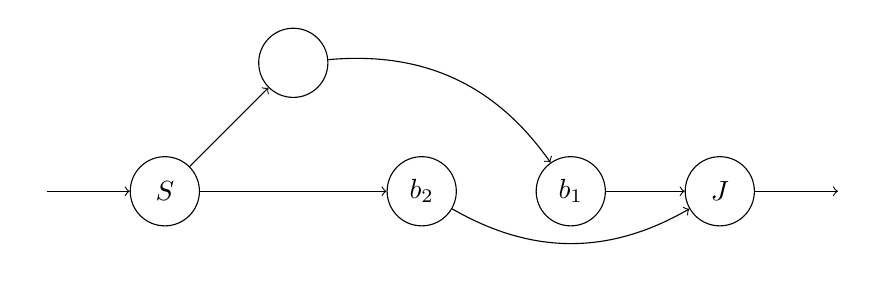
\begin{tikzpicture}
      [ initial text={}, initial distance=3em,
        accepting/.style=accepting by arrow,
        accepting distance=3em
      ]
      \node[state,initial]    (S)                              {$S$};
      \node[state]            (inside) [above right=of S]      {};
      \node[state]            (b_2)    [below right=of inside] {$b_2$};
      \node[state]            (b_1)    [right=of b_2]          {$b_1$};
      \node[state,accepting]  (J)      [right=of b_1]          {$J$};

      \path[->] (S)   edge              node  {}  (inside)
                      edge              node  {}  (b_2)
                (inside) edge [bend left] node {} (b_1)
                (b_1) edge              node  {}  (J)
                (b_2) edge [bend right] node  {}  (J);
    \end{tikzpicture}
  \end{subfigure}
  
  \caption{Cheating with go-tos}
  \label{fig:forbreak}
\end{figure}

\begin{figure}
  \ifstepb
  
  \whiletruestep
  \whilefalsestep
  \whileskipcontinuestep
  \whilebreakstep

  \labelstep

  \caption{Selected Conditional Steps}
  \label{fig:conditionals}
\end{figure}


When we step into a conditional or loop, we record its join point on the PC Tag, associated with the sources
that are tainted. Then, when we reach the label, we will subtract its sources from the PC Tag at that time.
This means that if multiple branches share a join point, their taints will be removed simultaneously.

\begin{minipage}[t]{.25\textwidth}
\[\begin{aligned}
\truledef{\splitt}
\settag{\PCT'}{\PCT[L \rightarrowtail \vt]}
\end{aligned}\]
\end{minipage}
\begin{minipage}[t]{.74\textwidth}
\[\begin{aligned}
\truledef{\joint}
\assert{\PCT = \mathit{pctaint} ~ \overline{(L,\sigma)}\}}
\settag{\PCT'}{\mathit{pctaint} ~ \{(L',\sigma) \mid (L',\sigma) \in \overline{(L,\sigma)} \land L \not \eq L'\}}
\end{aligned}\]
\end{minipage}

The \(\mathbf{JoinT}\) control point applies whenever we reach a labeled statement, seen
in \cref{fig:conditionals}.
The remaining branching constructs are rather complicated, involving multiple steps
and manipulations of the continuation that are not that relevant to their control
points. Rather than give their semantics in full, it suffices to identify which
transitions contain \(\mathbf{SplitT}\) control points. In \cref{fig:rest}, these
are the transitions from the state marked \(S\). Their semantics are given in full
in the appendix.

\begin{figure}
  \begin{subfigure}{0.5\textwidth}
    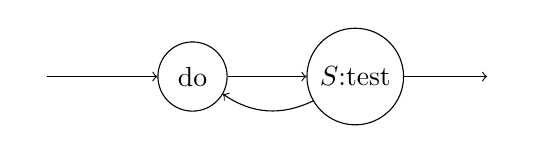
\begin{tikzpicture}
      [ initial text={}, initial distance=4em,
        accepting/.style=accepting by arrow,
        accepting distance=3em
      ]
      \node[state,initial]    (do)                             {do};
      \node[state,accepting]  (S) [right=of do]                {\(S\):test};

      \path[->] (do)   edge              node  {}  (S)
                (S)    edge [bend left]  node  {}  (do);
    \end{tikzpicture}
    \subcaption{Do-while}
  \end{subfigure}
  \begin{subfigure}{0.5\textwidth}
    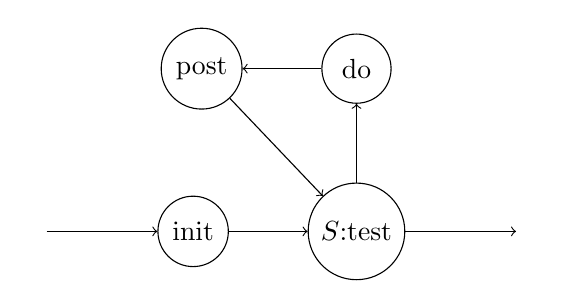
\begin{tikzpicture}
      [ initial text={}, initial distance=4em,
        accepting/.style=accepting by arrow,
        accepting distance=4em
      ]
      \node[state,initial]    (init)                             {init};
      \node[state,accepting]  (S)    [right=of init]             {\(S\):test};
      \node[state]            (do)   [above=of S]                {do};
      \node[state]            (post) [left=of do]                {post};
      
      \path[->] (init)   edge              node  {}  (S)
                (S)      edge              node  {}  (do)
                (do)     edge              node  {}  (post)
                (post)   edge              node  {}  (S);
    \end{tikzpicture}
    \subcaption{For}
  \end{subfigure}
  \begin{subfigure}{\textwidth}
    \center
    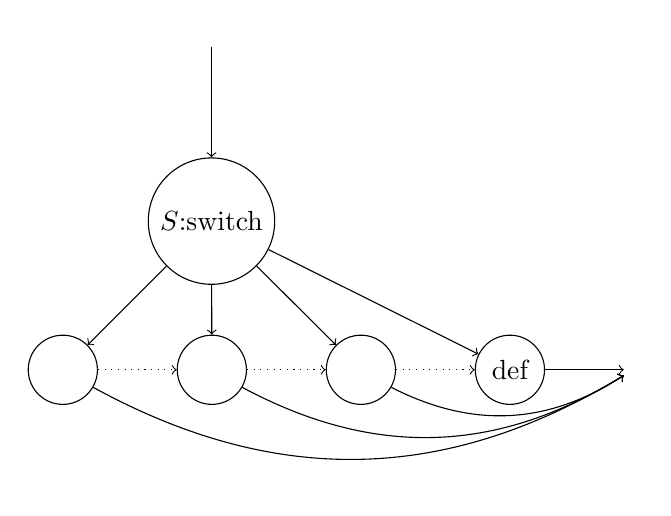
\begin{tikzpicture}
      [ initial text={}, initial distance=4em, initial above,
        accepting/.style=accepting by arrow,
        accepting distance=4em
      ]
      \node[state,initial]    (switch)                           {\(S\):switch};
      \node[state]            (case1)    [below left=of switch]  {};
      \node[state]            (case2)    [right=of case1]        {};
      \node[state]            (case3)    [right=of case2]        {};
      \node[state]            (default)  [right=of case3]        {def};
      \node                   (after)    [right=of default]      {};

      \path[->] (switch)  edge              node  {}  (case1)
                          edge              node  {}  (case2)
                          edge              node  {}  (case3)
                          edge              node  {}  (default)
                (default) edge              node  {}  (after)
                (case1)   edge [bend right] node  {}  (after)
                (case2)   edge [bend right] node  {}  (after)
                (case3)   edge [bend right] node  {}  (after);

      \path[dotted,->] (case1) edge              node  {}  (case2)
                (case2) edge              node  {}  (case3)
                (case3) edge              node  {}  (default);
                         
    \end{tikzpicture}
    \subcaption{Switch}
  \end{subfigure}

  
  
  \caption{Remaining Branch Statements}
  \label{fig:rest}
\end{figure}

\paragraph*{Realizing IFC}

In order to implement an IFC policy, we need to specify the rules that it needs to enforce.
The positive here is that the rules are not dependent on one another (with the exception of
declassification rules), and default to permissiveness when no rule is given. We assume that
the user would supply a separate file consisting of a list of triples: the source, the sink,
and the type of rule. This is then translated into the policy.

The other implementation detail to consider are the label tags. These resemble
instruction tags, and that is exactly how they would be implemented: as a special instruction
tag on the appropriate instruction, which might be an existing instruction or a specially
added no-op. But importantly, in this case, these tags are mutable; in a policy that can be
expected to take advantage of their mutability, we will need an extra store to set the tag
for later.

It remains to generate those labels. For purposes of an IFC policy, we first generate the program's
control flow graph. Then, for each if, while, do-while, for, and switch statement, we identify the
immediate post-dominator in the graph, and wrap it in a label statement with a fresh identifier.
That identifier is also added as a field in the original conditional statement. The tags
associated with the labels are initialized at program state---in the case of IFC, these defaults
declare that there are no secrets to lowre when it is reached.

\section{Compartmentalization}
\label{sec:comp}

Coverity has examples of:
``all the old stuff goes over there, new code has stricter requirements.''

\section{Evaluation}
\label{sec:evaluation}

\section{Related and Future Work}
\label{sec:relwork}

\bibliography{taggedc.bib}

\appendix

\section{Continuations}
\label{app:continuations}

\[\begin{split}
\cont ::= & \kemp \\
| & \kdo{\cont} \\
| & \kseq{\stmt}{\cont} \\
| & \kif{\stmt_1}{\stmt_2}{L}{\cont} \\
| & \kwhiletest{\expr}{\stmt}{L}{\cont} \\
| & \kwhileloop{\expr}{\stmt}{L}{\cont} \\
| & \kdowhiletest{\expr}{\stmt}{L}{\cont} \\
| & \kdowhileloop{\expr}{\stmt}{L}{\cont} \\
| & \kfor{\stmt}{\cont} \\
| & \kforpost{\stmt}{\cont} \\
\end{split}\]

\section{Step rules}
\label{app:rules}

\subsection{Sequencing rules}

\dostepa
\dostepb
\seqstep
\seqskipstep
\seqcontinuestep
\seqbreakstep
\retvalstep
\labelstep

\subsection{Conditional rules}

\ifstepa
\ifstepb

TODO: switch

\subsection{Loop rules}

%% While %%
\whilestep
\whiletruestep
\whilefalsestep
\whileskipcontinuestep
\whilebreakstep

%% Do-while %%
\dowhilestep
\dowhileskipcontinuestep
\dowhilefalsestep
\dowhiletruestep
\dowhilebreakstep

%% For %%
\forinitstep
\forstep
\forfalsestep
\fortruestep
\forskiporcontinuestep
\forbreakstep
\forskippoststep

\subsection{Expression Rules}

\allocstep
\valofstep
\assignopstep
\postincstep
\assignstep
\varstep
\unopstep
\binopstep
\callexprstep

\subsection{Call and Return Rules}

\callstep
\returnstep

\end{document}
